\documentclass[10pt,twocolumn]{article}
\usepackage[a4paper,margin=1.8cm,columnsep=0.6cm]{geometry}
\usepackage[T1]{fontenc}
\usepackage[utf8]{inputenc}
\usepackage{lmodern}
\usepackage{mathptmx}
\usepackage{amsmath,amssymb}
\usepackage{microtype}
\usepackage{graphicx}
\usepackage{booktabs}
\usepackage{multirow}
\usepackage{siunitx}
\usepackage{xcolor}
\usepackage{tikz}
\usetikzlibrary{positioning,arrows.meta,fit,backgrounds,calc,decorations.pathreplacing,shapes.misc,matrix}
\usepackage{pgfplots}
\pgfplotsset{compat=1.18}
\usepackage[numbers,sort&compress]{natbib}
\usepackage[hidelinks]{hyperref}
\usepackage[capitalise,noabbrev]{cleveref}
\usepackage{caption}
\usepackage{float}
\captionsetup{font=small,labelfont=bf}
\sisetup{detect-all,group-minimum-digits=4}

% shared colours and TikZ styles for the paper's figures
\definecolor{model}{HTML}{2a78d6}
\definecolor{rule}{HTML}{eb6834}
\definecolor{muted}{HTML}{52514e}
\definecolor{deep}{HTML}{7b4fc2}
\definecolor{sup}{HTML}{1a9a7a}
\definecolor{faint}{HTML}{e9e8e4}
\tikzset{
  >={Stealth[length=4pt]},
  box/.style={draw=muted, rounded corners=2pt, align=center, inner sep=3pt, fill=white, font=\footnotesize},
  arr/.style={->, draw=muted, line width=0.6pt},
  note/.style={draw=muted!60!black, fill=muted!75, rounded corners=0.6pt, minimum width=0.42cm, minimum height=0.11cm, inner sep=0pt},
  lnbody/.style={draw=muted!60!black, fill=muted!25, rounded corners=0.6pt},
  lbl/.style={font=\scriptsize, text=muted, align=left},
  cell/.style={draw=muted!50, minimum size=0.17cm, inner sep=0pt},
  on/.style={fill=muted!80},
}

% generated by paper/experiments/v2_tables.py
\newcommand{\catRule}{0.564}
\newcommand{\tagRule}{0.452}
\newcommand{\catBase}{0.719}
\newcommand{\tagBase}{0.588}
\newcommand{\catBoost}{0.749}
\newcommand{\tagBoost}{0.616}
\newcommand{\catMlp}{0.747}
\newcommand{\tagMlp}{0.625}
\newcommand{\catDeep}{0.751}
\newcommand{\tagDeep}{0.625}
\newcommand{\catWide}{0.762}
\newcommand{\tagWide}{0.629}
\newcommand{\catEns}{0.768}
\newcommand{\tagEns}{0.636}
\newcommand{\catGain}{+0.049}
\newcommand{\tagGain}{+0.047}
\newcommand{\catBeatsBase}{11}
\newcommand{\tagBeatsBase}{20}
\newcommand{\nPlain}{3}
\newcommand{\nWide}{6}
\newcommand{\nCharts}{36{,}509}
\newcommand{\nSongs}{11{,}376}
\newcommand{\nUnlab}{26{,}536}
\newcommand{\catNoSv}{0.756}
\newcommand{\tagNoSv}{0.635}
\newcommand{\apMemoBase}{0.27}
\newcommand{\apMemoEns}{0.53}
\newcommand{\apMemoNoSv}{0.41}
\newcommand{\apMemoBoostNoSv}{0.27}
\newcommand{\apMemoBoostSv}{0.44}
\newcommand{\apReadingBase}{0.89}
\newcommand{\apReadingEns}{0.91}
\newcommand{\apReadingNoSv}{0.91}
\newcommand{\apReadingBoostNoSv}{0.91}
\newcommand{\apReadingBoostSv}{0.91}
\newcommand{\catLo}{+0.036}
\newcommand{\catHi}{+0.060}
\newcommand{\catShare}{0.38}
\newcommand{\tagLo}{+0.040}
\newcommand{\tagHi}{+0.055}
\newcommand{\tagShare}{0.25}
\newcommand{\nBoot}{500}

\newcommand{\utag}[1]{\texttt{\small #1}}
\newcommand{\RC}{\textsc{rc}}
\newcommand{\LN}{\textsc{ln}}
\newcommand{\HB}{\textsc{hb}}
\newcommand{\SV}{\textsc{sv}}

\title{\bfseries Learning Tournament Slots and Pattern Skillsets of osu!mania Charts\\from Expert Mappools and Crowd-Sourced Tags}
\author{Komi\\\small\texttt{j.ruza@udc.es}}
\date{}

\begin{document}
\maketitle

\begin{abstract}
Players and tournament organisers describe osu!mania charts in a shared vocabulary of \emph{slots} (rice, long note, hybrid, scroll speed) and \emph{skillsets} (jumpstream, chordjack, LN release, \dots). Beatmap Nominators, who triage far more ranking requests than they can play, would benefit from an automatic description in these terms. We build one from public data only. The mappools of 115 official tournaments label the slot of \num{4029} charts, and crowd-voted user tags on all \num{30732} ranked osu!mania difficulties label skillsets, which we treat as positive--unlabelled data with a strict and a relaxed threshold. A chart is represented twice: as one interpretable vector (71 statistics, their distribution over 16-second windows, a bag of row transitions, \emph{reading} features that describe what scroll-speed changes do to the notes on screen, and MinaCalc skillset ratings), and as a sequence of note events. A gradient-boosted classifier on the statistics predicts the tournament slot with 98.1\% accuracy, against 88.5\% for slotting rules. For 11 reviewer categories and 20 user tags we average four model families: boosted heads, a multi-task MLP, and two event encoders (dilated convolutions and a transformer over 4-second windows, with attention-based multiple-instance heads) that are pretrained with masked-event and masked-window objectives and distilled from per-fold teachers on the \nUnlab{} charts without a strict label. Under cross-validation grouped by song over all \nCharts{} charts, in which no model sees any chart of a test song, the ensemble reaches a mean average precision of \catEns{} on the categories and \tagEns{} on the tags, against \catBase{} and \tagBase{} for a boosted head on statistics and windows ($\catGain$ and $\tagGain$; 95\% song-bootstrap intervals $[\catLo, \catHi]$ and $[\tagLo, \tagHi]$).
\end{abstract}

% =====================================================================
\section{Introduction}

osu! is a free rhythm game with a large community of chart authors (\emph{mappers}). Its osu!mania mode is a vertical-scrolling key game in the tradition of Beatmania and StepMania: notes fall down $K$ columns ($K\in\{4,7\}$ in most play) and must be hit, or for \emph{long notes} (LNs) held and released, in time with the music. A chart (\emph{difficulty}) enters the ranked section only after two Beatmap Nominators (BNs) review and nominate it. BNs receive far more requests than they can play, and choose what to check largely by what kind of chart it is.

The community has a precise, if informal, vocabulary for that. Tournament mappools group charts into \emph{slots}, of which four are near-universal: \emph{rice} (\RC; tap notes), \emph{long note} (\LN), \emph{hybrid} (\HB; a mix of both) and \emph{scroll speed} (\SV; charts whose difficulty comes from changing scroll velocity). Within a slot, players speak of \emph{skillsets}: jumpstream, handstream, chordjack, speed jacks, technical rhythm, stamina, LN release, LN coordination, inverse LNs, reading and memorising scroll changes, and so on. A reviewer who knows that a request is ``a 4K hybrid with dense inverse LNs and technical rhythm'' can route or prioritise it without opening it.

Producing that description automatically raises three problems. \emph{Labels}: there is no annotated dataset. Tournament organisers slot charts carefully but only at the slot level; osu!(lazer) lets players vote \emph{user tags} on charts they have passed, which gives skillset labels, but only for ranked charts with an audience, and only positively: a tag nobody voted for is not evidence that the pattern is absent. \emph{Representation}: charts vary in key count, length, tempo and note count by orders of magnitude; the skillsets of interest are defined on short local configurations (a jack is the same column hit twice in quick succession); and some of them, such as an LN release section in a rice chart, occupy only part of the chart. \emph{Evaluation}: tournament pools contain rate-altered copies of one song and a ranked beatmapset contains several difficulties of the same song, so random splits leak, and unlabelled charts used for pretraining or distillation can leak too.

This paper describes a system that addresses each in turn (\cref{fig:pipeline}). Our contributions are:
\begin{itemize}\setlength\itemsep{1pt}
\item Weakly supervised datasets built from public pages only: tournament slots for \num{4029} charts, and strict and relaxed skillset labels for 11 reviewer categories and 20 user tags, derived from user-tag votes and tournament sub-slots (\cref{sec:data}).
\item Two complementary chart representations: an interpretable vector of chart statistics, window statistics, row transitions, reading features and MinaCalc ratings, and a tokenisation of the chart into note events (\cref{sec:features}).
\item A slot classifier, and an ensemble of four model families for the categories and tags, in which neural students learn from unlabelled charts through per-fold teachers and self-supervised objectives without ever seeing a test song (\cref{sec:models}).
\item An evaluation grouped by song over the whole corpus, with paired song-bootstrap intervals, against rule baselines and a boosted reference on identical charts (\cref{sec:results}).
\end{itemize}

\begin{figure*}[t]
\centering
\resizebox{\textwidth}{!}{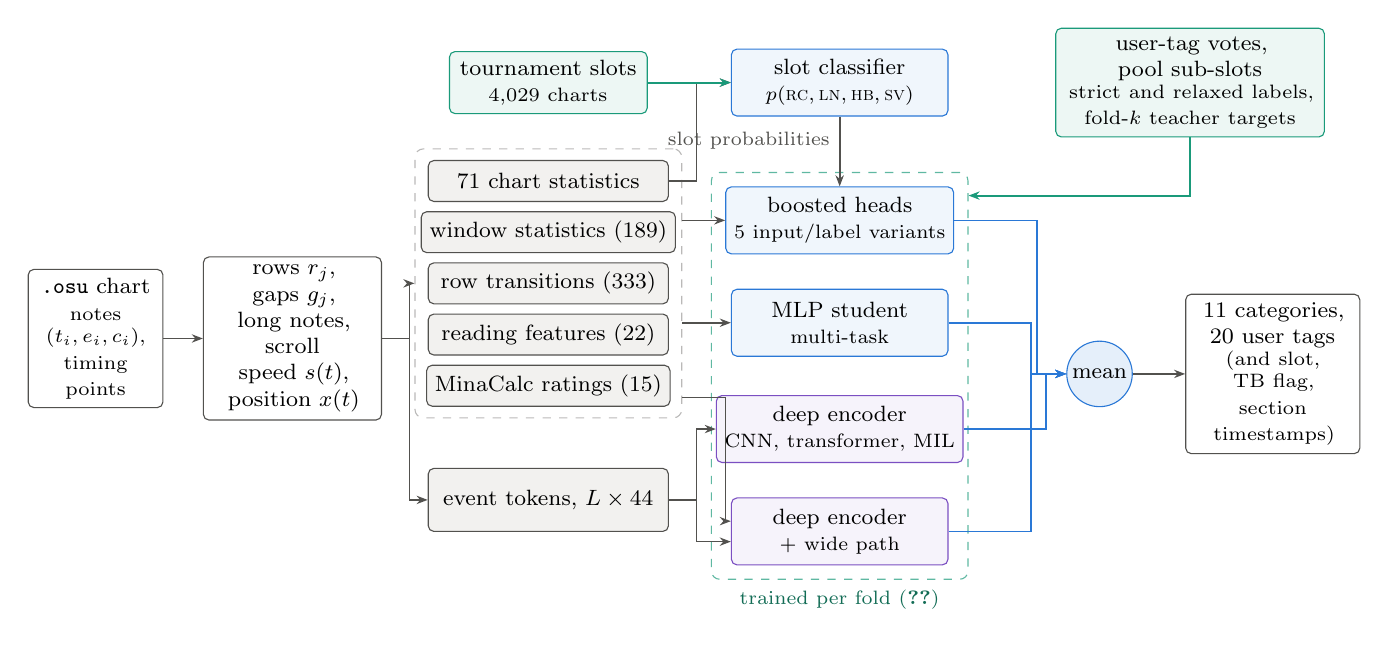
\begin{tikzpicture}[
  feat/.style={box, minimum width=3.05cm, minimum height=0.52cm, fill=faint!60},
  mdl/.style={box, minimum width=2.75cm, minimum height=0.85cm, draw=model, fill=model!7},
  dmdl/.style={mdl, draw=deep, fill=deep!7},
  sup/.style={box, draw=sup, fill=sup!8},
  sarr/.style={arr, draw=sup, line width=0.7pt}]
% input and parsing
\node[box, text width=1.5cm, minimum height=1.45cm] (osu) at (0,0.6) {\texttt{.osu} chart\\[2pt]{\scriptsize notes $(t_i,e_i,c_i)$,\\timing points}};
\node[box, text width=2.05cm, minimum height=1.45cm] (parse) at (2.5,0.6) {rows $r_j$, gaps $g_j$,\\long notes,\\scroll speed $s(t)$,\\position $x(t)$};
% features
\node[feat] (stats) at (5.75,2.6) {71 chart statistics};
\node[feat] (win)   at (5.75,1.95) {window statistics (189)};
\node[feat] (pat)   at (5.75,1.3) {row transitions (333)};
\node[feat] (read)  at (5.75,0.65) {reading features (22)};
\node[feat] (msd)   at (5.75,0.0) {MinaCalc ratings (15)};
\node[feat, minimum height=0.8cm, align=center] (tok) at (5.75,-1.45) {event tokens, $L\times 44$};
\begin{scope}[on background layer]
\node[draw=muted!40, dashed, rounded corners=3pt, fit=(stats)(msd), inner sep=4pt] (fbox) {};
\end{scope}
% models
\node[mdl] (slot) at (9.45,3.85) {slot classifier\\{\scriptsize $p(\RC,\LN,\HB,\SV)$}};
\node[mdl] (boost) at (9.45,2.1) {boosted heads\\{\scriptsize 5 input/label variants}};
\node[mdl] (mlp) at (9.45,0.8) {MLP student\\{\scriptsize multi-task}};
\node[dmdl] (deep) at (9.45,-0.55) {deep encoder\\{\scriptsize CNN, transformer, MIL}};
\node[dmdl] (wide) at (9.45,-1.85) {deep encoder\\{\scriptsize + wide path}};
\begin{scope}[on background layer]
\node[draw=sup!70, dashed, rounded corners=3pt, fit=(boost)(wide), inner sep=5pt] (frame) {};
\end{scope}
\node[lbl, text=sup!70!black, anchor=north] at (frame.south) {trained per fold (\cref{fig:protocol})};
% supervision
\node[sup, text width=2.3cm] (pools) at (5.75,3.85) {tournament slots\\{\scriptsize 4{,}029 charts}};
\node[sup, text width=3.2cm] (tags) at (13.9,3.85) {user-tag votes, pool sub-slots\\{\scriptsize strict and relaxed labels,\\fold-$k$ teacher targets}};
% ensemble and output
\node[circle, draw=model, fill=model!12, inner sep=1.5pt, font=\footnotesize] (mean) at (12.75,0.15) {mean};
\node[box, text width=2.0cm, minimum height=1.3cm] (out) at (14.95,0.15) {11 categories,\\20 user tags\\{\scriptsize (and slot, TB flag,\\section timestamps)}};
% arrows: parsing and features
\draw[arr] (osu) -- (parse);
\draw[arr] (parse.east) -- ++(0.35,0) |- (fbox.west);
\draw[arr] (parse.east) -- ++(0.35,0) |- (tok.west);
\draw[arr] (stats.east) -- ++(0.35,0) |- (slot.west);
\draw[arr] (boost.west -| fbox.east) -- (boost.west);
\draw[arr] (mlp.west -| fbox.east) -- (mlp.west);
\draw[arr] ([yshift=-1.5mm]msd.east -| fbox.east) -- ++(0.55,0) |- ([yshift=1.3mm]wide.west);
\draw[arr] (tok.east) -- ++(0.35,0) |- (deep.west);
\draw[arr] (tok.east) -- ++(0.35,0) |- ([yshift=-1.3mm]wide.west);
\draw[arr] (slot) -- node[lbl, left, pos=0.35] {slot probabilities} (boost);
% supervision arrows
\draw[sarr] (pools) -- (slot);
\draw[sarr] (tags.south) |- ([yshift=-3mm]frame.north east);
% ensemble arrows
\foreach \m in {boost, mlp, deep, wide} \draw[arr, draw=model] (\m.east) -- ++(1.05,0) |- (mean.west);
\draw[arr] (mean) -- (out);
\end{tikzpicture}
}
\caption{The system. A chart is parsed into rows, long notes and a scroll profile, and represented both as one vector of interpretable features per chart and as a sequence of note events. A boosted classifier trained on tournament slots predicts the slot. Four model families predict the reviewer categories and user tags and are averaged: boosted heads and an MLP on the feature vector, and two event encoders, one of which also sees the feature vector through a wide path. Green: supervision.}
\label{fig:pipeline}
\end{figure*}

% =====================================================================
\section{Background and related work}\label{sec:related}

\paragraph{osu!mania charts.} A chart is a list of hit objects $(t_i, e_i, c_i)$ with start time $t_i$, end time $e_i\ge t_i$ ($e_i>t_i$ for an LN) and column $c_i\in\{0,\dots,K-1\}$, plus a list of \emph{timing points}. Uninherited (``red'') points set the beat length and hence the BPM; inherited (``green'') points set a slider-velocity (SV) multiplier that, in osu!mania, scales how fast notes scroll. Together they determine an effective scroll speed that may differ greatly from the song's tempo; \SV{} charts exploit this.

\paragraph{Difficulty and pattern analysis.} osu!'s own star rating is a hand-designed strain model that outputs a single number. Etterna's MinaCalc rates charts per skillset (stream, jumpstream, handstream, stamina, jackspeed, chordjack, technical) with hand-tuned pattern detectors \citep{minacalc}; we use its ratings as features. Community tools for osu! are also rule-based: \citet{rosupattern} detect mania jacks and jump/hand streams, while SimpleBeatmapAnalyzer \citep{simplebeatmap} and osu-finder \citep{osufinder} classify osu!standard maps by spacing or strain ratios. None learns from labels or outputs tournament slots. Our rule baselines (\cref{sec:rules}) are in the spirit of these tools.

\paragraph{Machine learning on rhythm-game charts.} Most learned work generates charts from audio: Dance Dance Convolution \citep{donahue2017ddc} and its successors \citep{yi2023beataligned,an2026transfer}, and TaikoNation, which targets human-like patterning \citep{halina2021taikonation}. \citet{franks2023ordinal} estimate StepMania difficulty levels with ordinal regression, and \citet{liu2025osu2mir} use osu! timing as beat-tracking labels. To our knowledge no prior work classifies charts into tournament slots or predicts crowd skillset tags.

\paragraph{Learning from tags and positive-only labels.} Predicting user tags is analogous to music auto-tagging \citep{lamere2008social,choi2016autotagging}, where social tags are sparse and under-reported \citep{golder2006usage}. A missing tag is an unlabelled example rather than a negative one, the setting of positive--unlabelled (PU) learning \citep{elkan2008pu,bekker2020pu} and of multi-label learning with missing labels \citep{yu2014missing}. We abstain on insufficiently annotated charts and down-weight weakly annotated ones; combining several noisy label sources by rules is a form of weak supervision \citep{ratner2017snorkel}.

\paragraph{Models.} The boosted heads are gradient-boosted trees \citep{friedman2001gbm} in the histogram formulation of LightGBM \citep{ke2017lightgbm} as implemented in scikit-learn \citep{pedregosa2011sklearn}, which remain strong on tabular data \citep{grinsztajn2022tree}; feeding rule scores to them is stacking \citep{wolpert1992stacked}. The neural students are trained on teacher probabilities where labels are missing, which is knowledge distillation \citep{hinton2015distilling} used for self-training on unlabelled data \citep{xie2020noisy}. The event encoder combines gated \citep{dauphin2017glu} dilated \citep{oord2016wavenet} convolutions with a transformer \citep{vaswani2017attention}, is pretrained by masked prediction \citep{devlin2019bert}, and reads out each label with attention-based multiple-instance pooling \citep{dietterich1997mil,ilse2018attention}, since a chart is positive for a skillset when some of its sections are. Its wide path follows wide-and-deep models \citep{cheng2016wide}, and the final prediction is a plain ensemble average \citep{dietterich2000ensemble}. Group-aware cross-validation avoids the leakage that related samples cause \citep{kaufman2012leakage,roberts2017cv}.

% =====================================================================
\section{Data}\label{sec:data}

Everything is collected without an osu! API key: the osu! wiki is a public Git repository, chart files are served at \texttt{osu.ppy.sh/osu/\{id\}}, and the public beatmapset page embeds the same JSON the API returns, including each difficulty's user tags with vote counts.

\subsection{Tournament mappools (slot labels)}\label{sec:pools}
The osu! wiki documents the mappools of officially supported tournaments. We parsed \num{9963} pool entries (\num{8454} distinct charts) from 115 osu!mania tournaments in 42 series (e.g.\ MWC, MCNC, 4DM, SOFT, o!mLN, JHC) and downloaded every chart. A normaliser maps raw slot names (``LN'', ``Long Note'', ``Long Notes'') onto $\mathcal{Y}=\{\RC,\LN,\HB,\SV\}$; tournaments that are wholly one category inherit it (all of o!mLN is \LN, all of SVSE is \SV, and the jack-and-chord tournament JHC is \RC). FreeMod, NoMod, Tiebreaker and Wildcard slots carry no pattern information and are left unlabelled. A chart in several pools receives the majority label and exact ties are discarded. After removing charts with fewer than 50 notes or fewer than 4 keys, \num{4029} charts of \num{3558} songs are labelled. Sub-slot names (``Dense Chordjack'', ``Coordination'', ``Memorisation'', ``Tiebreaker'') are kept for the categories of \cref{sec:categories}.

\subsection{User tags on ranked charts (skillset labels)}\label{sec:tags-data}
We listed all \num{8673} ranked osu!mania beatmapsets and fetched the user tags of their \num{30732} difficulties. Votes are sparse: \num{10031} difficulties have at least one vote and \num{3227} have eight or more. Let $v_{d,\tau}$ be the number of votes for tag $\tau$ on difficulty $d$ and $V_d=\sum_\tau v_{d,\tau}$. The \emph{strict} label, used for training and for all evaluation, is
\begin{equation}
y_{d,\tau}=\begin{cases}1 & v_{d,\tau}\ge 2,\\ 0 & v_{d,\tau}=0\text{ and }V_d\ge 8,\\ \varnothing & \text{otherwise,}\end{cases}
\label{eq:labels}
\end{equation}
where $\varnothing$ (unknown) removes the pair from that tag's training and evaluation sets: a single vote is often idiosyncratic, and a difficulty with few votes says little about the tags it lacks. The \emph{relaxed} label adds, for training only and at weight $\tfrac12$, the pairs that \cref{eq:labels} leaves unknown but that carry some evidence: $y=1$ if $v_{d,\tau}=1$, and $y=0$ if $v_{d,\tau}=0$ and $3\le V_d\le7$. We keep the 20 mania tags with at least 12 strict positives and 12 strict negatives (\cref{tab:v2-tags}).

\subsection{Reviewer categories}\label{sec:categories}
The BN who requested this tool defined the categories in which predictions are reported (multi-label): \emph{Rice}: Chordjack, Streams, Jumpstream/Handstream, Technical, Mixed Rice, Stamina; \emph{LN}: Release, Coordination, Density/Inverse; \emph{SV}: Reading, Memo; \emph{Hybrid}; and \emph{TB} (tiebreaker-worthy). Hybrid is the slot of \cref{sec:pools}, and Mixed Rice is derived: a chart is Mixed Rice when skills from at least two of the families \{Chordjack\}, \{Streams, Jumpstream/Handstream\}, \{Technical\} fire. The other 11 categories have learned heads and draw labels from two sources, combined by ``positive anywhere wins, otherwise negative anywhere, otherwise unknown'':
\begin{itemize}\setlength\itemsep{1pt}
\item user tags, through a fixed many-to-one map (e.g.\ Jumpstream/Handstream $\leftarrow$ \utag{style/jumpstream}, \utag{style/handstream}, \utag{style/chordstream}, \utag{style/quadstream}) with \cref{eq:labels} applied to the category's most-voted tag, and the relaxed rule likewise;
\item tournament sub-slots (JHC's chordjack and quadstream slots, o!mLN's Coordination and Density, SVSE's Reading and Memorisation, and every pool's Tiebreaker). A chart in one sub-slot is a negative for the sibling sub-slots of the same tournament, because poolers slot by the dominant skill; for TB, every other slot-labelled pool chart is a negative.
\end{itemize}
Two mappings needed care. The mania tag \utag{skillset/reading} denotes reading dense patterns rather than scroll-speed reading, so SV Reading uses the \utag{sliders/*} tags. Memo uses \utag{gimmick/memory}, but only on charts whose scroll speed actually varies, since the tag is also voted on storyboard gimmicks.

\subsection{Corpus and folds}\label{sec:corpus}
The category and tag experiments use every ranked osu!mania chart together with every tournament chart we could download, \nCharts{} charts in all (\cref{tab:v2-data}). Most of them have no strict label for any task; they are still useful, as inputs for self-supervised pretraining and as charts on which a teacher's predictions can be distilled. To make that safe, the five cross-validation folds are drawn by \emph{song} over the whole corpus: the song key is the normalised artist and title with mapper and difficulty names stripped, so rate edits, re-uploads and the difficulties of a beatmapset stay together. A model for fold $k$ never sees any chart of a fold-$k$ song, labelled or not.

\begin{table}[t]
\centering\small
\caption{The chart corpus of the category and tag experiments. Every chart is assigned to one of five folds by its song; a model for fold $k$ never sees a chart of a fold-$k$ song.}
\label{tab:v2-data}
\begin{tabular}{lr}
\toprule
Charts in the corpus & \num{36509} \\
\quad in a tournament pool & \num{7251} \\
\quad ranked, not pooled & \num{29258} \\
Songs (fold groups) & \num{11376} \\
\midrule
Charts with $\ge1$ strict category label & \num{9559} \\
Charts with $\ge1$ strict tag label & \num{5640} \\
Charts with no strict label & \num{26536} \\
Relaxed (chart, task) labels added & \num{102725} \\
\quad of which positive & \num{11519} \\
\bottomrule
\end{tabular}
\end{table}


% =====================================================================
\section{Chart representation}\label{sec:features}

\subsection{Rows, gaps and scroll position}\label{sec:rows}
Notes whose start times lie within \SI{2}{ms} form a \emph{row} $r_j$ at time $\tau_j$ with column set $C_j$. Let $g_j=\tau_j-\tau_{j-1}$; a transition is \emph{fast} if $g_j<\SI{220}{ms}$, inside a pattern rather than a pause. The timing points define a piecewise-constant effective scroll speed
\begin{equation}
s(t)=\frac{\beta_{\text{main}}}{\beta(t)}\,\mathrm{sv}(t),
\end{equation}
where $\beta(t)$ is the active beat length, $\beta_{\text{main}}$ the beat length covering most of the chart, and $\mathrm{sv}(t)\in[0.01,10]$ the active SV multiplier, reset to 1 at each red point. Its integral $x(t)=\int_0^t s(u)\,du$ is the \emph{scroll position}: a note hit at time $T$ is drawn at height $x(T)-x(t)$ above the judgement line at time $t$.

\subsection{Chart statistics}\label{sec:stats}
71 statistics describe the chart as a whole, each a quantity a mappooler inspects (\cref{fig:features}a; full list in \cref{app:features}). They are normalised by note count, row count or duration so that charts of different key counts and lengths are comparable, and $K$ is itself a feature.
\textbf{Meta and density} (15): keys, OD, HP, note count, duration, notes per second overall and per key, percentiles of 2-second note rates, peak-to-median ratio, a stamina proxy (the share of windows within 80\% of the 90th-percentile rate) and the variation of density.
\textbf{Chords, jacks and streams} (22): shares of single, jump, hand and quad rows; the share of fast transitions with $C_j\cap C_{j-1}\neq\emptyset$ (\emph{jack rows}), of jack rows between two chords (\emph{chordjacks}) and of fast transitions with $C_j\cap C_{j-1}=\emptyset$ (\emph{stream rows}), split into jumpstream and handstream by $|C_j|$; jack gaps and chains; trills; and anchors.
\textbf{Rhythm} (14): the distribution of the snap of fast gaps relative to the local beat (1/2 to 1/16, triplets, other), the number of distinct gaps per 16 rows, the rate of large gap-ratio changes, the main BPM and the number of BPMs.
\textbf{Long notes} (11): LN share $\rho$, LNs per second, LN lengths in ms and beats, hold coverage $\sum_i(e_i-t_i)/(K\cdot T)$, the inverse rate (an LN followed in its column by a note less than 0.3 beats after its release), the share of releases on no row (\emph{off-grid}), and the mean number of columns held while a note is hit, divided by $K$ (\emph{coordination}).
\textbf{Scroll speed} (9): the duration-weighted standard deviation $\sigma_{\log s}$ of $\log s$, the share of time with $|\log s|>0.05$ and $>0.4$, of near-stops ($s<0.2$) and fast sections ($s>2$), SV point and change rates, and the rate of SV changes within \SI{1.5}{s} of a note.

\begin{figure*}[t]
\centering
\resizebox{\textwidth}{!}{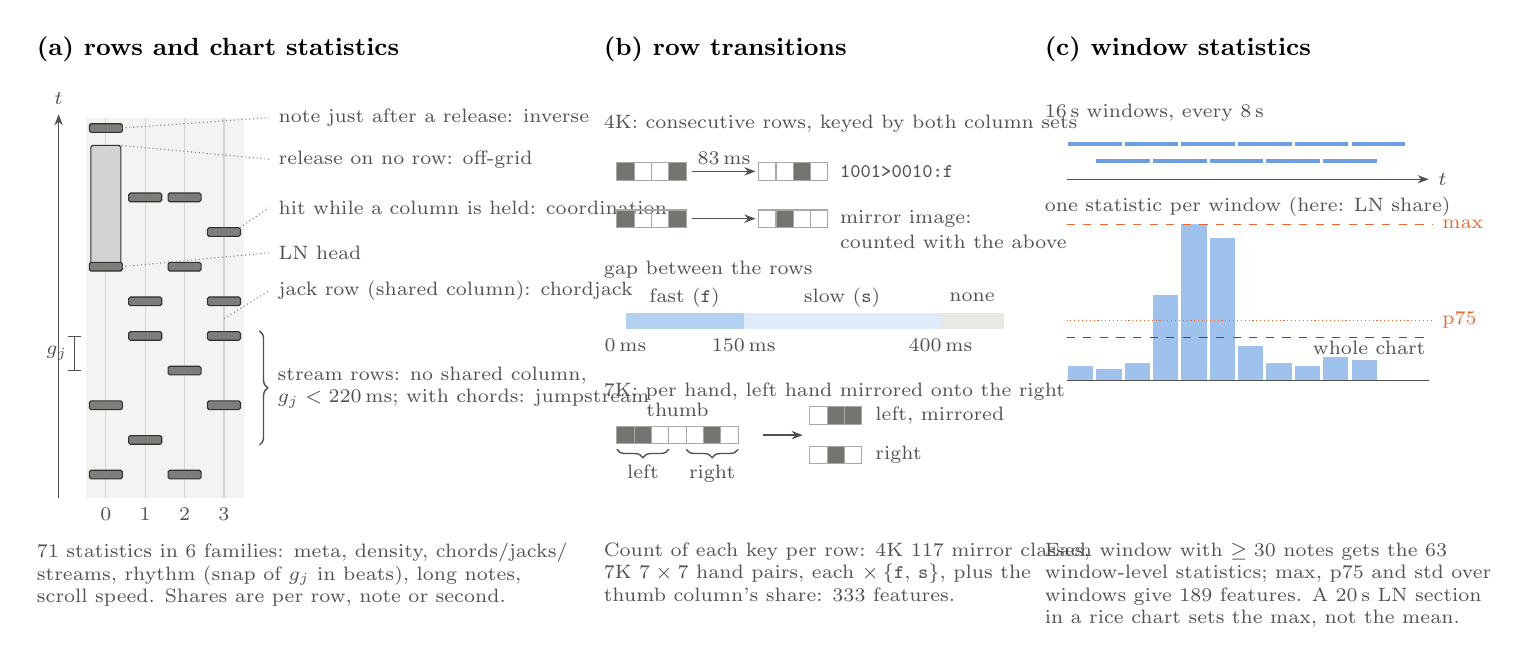
\begin{tikzpicture}[
  ycell/.style={cell, minimum size=0.16cm},
  brace/.style={decorate, decoration={brace, amplitude=3pt}, draw=muted, line width=0.5pt}]
% ================= (a) rows and chart statistics =================
\begin{scope}
\def\dx{0.5}\def\dy{0.44}
\node[font=\small\bfseries, anchor=west] at (-1.0,5.4) {(a) rows and chart statistics};
% playfield
\fill[faint!50] (-0.25,-0.3) rectangle (1.75,10.3*\dy);
\foreach \c in {0,...,3} \draw[muted!25] ({\c*\dx},-0.3) -- ({\c*\dx},10.3*\dy);
\foreach \c in {0,...,3} \node[lbl] at ({\c*\dx},-0.5) {\c};
% long note in column 0 from t=6 to t=9.5
\draw[lnbody] ({-0.19},{6*\dy}) rectangle ({0.19},{9.5*\dy});
% rows: t / columns
\foreach \t/\cs in {0/{0,2}, 1/{1}, 2/{0,3}, 3/{2}, 4/{1,3}, 5/{1,3}, 6/{0,2}, 7/{3}, 8/{1,2}, 10/{0}} {
  \foreach \c in \cs \node[note] at ({\c*\dx},{\t*\dy}) {};
}
% time axis and a gap
\draw[->, muted] (-0.6,-0.3) -- (-0.6,10.4*\dy) node[lbl, above] {$t$};
\draw[muted, |-|] (-0.4,{3*\dy}) -- node[lbl, left=-1pt] {$g_j$} (-0.4,{4*\dy});
% annotations
\def\ax{1.95}
\draw[brace] (\ax,{4.15*\dy}) -- (\ax,{0.85*\dy}) node[lbl, midway, right=3pt] {stream rows: no shared column,\\$g_j<220$\,ms; with chords: jumpstream};
\node[lbl, right] (jk) at (\ax+0.12,{5.3*\dy}) {jack row (shared column): chordjack};
\node[lbl, right] (lh) at (\ax+0.12,{6.4*\dy}) {LN head};
\node[lbl, right] (co) at (\ax+0.12,{7.7*\dy}) {hit while a column is held: coordination};
\node[lbl, right] (og) at (\ax+0.12,{9.1*\dy}) {release on no row: off-grid};
\node[lbl, right] (iv) at (\ax+0.12,{10.3*\dy}) {note just after a release: inverse};
\draw[muted!70, densely dotted] (1.5,{4.5*\dy}) -- (jk.west);
\draw[muted!70, densely dotted] (0.2,{6*\dy}) -- (lh.west);
\draw[muted!70, densely dotted] (1.62,{7*\dy}) -- (co.west);
\draw[muted!70, densely dotted] (0.2,{9.5*\dy}) -- (og.west);
\draw[muted!70, densely dotted] (0.2,{10*\dy}) -- (iv.west);
\node[lbl, align=left, anchor=north west] at (-1.0,-0.75) {71 statistics in 6 families: meta, density, chords/jacks/\\streams, rhythm (snap of $g_j$ in beats), long notes,\\scroll speed. Shares are per row, note or second.};
\end{scope}
% ================= (b) row transitions =================
\begin{scope}[xshift=6.6cm]
\node[font=\small\bfseries, anchor=west] at (-0.4,5.4) {(b) row transitions};
\newcommand{\row}[3]{% x y bits
  \foreach \b [count=\i from 0] in {#3} {
    \node[ycell, minimum size=0.22cm] at ({#1+\i*0.22},#2) {};
    \ifnum\b=1 \node[ycell, on, minimum size=0.22cm] at ({#1+\i*0.22},#2) {}; \fi
  }}
% a 4K pair
\node[lbl, anchor=west] at (-0.4,4.45) {4K: consecutive rows, keyed by both column sets};
\row{0}{3.85}{1,0,0,1}
\draw[arr] (0.85,3.85) -- node[lbl, above=-1pt] {83\,ms} (1.65,3.85);
\row{1.8}{3.85}{0,0,1,0}
\node[lbl, right] at (2.6,3.85) {\texttt{1001>0010:f}};
\row{0}{3.25}{1,0,0,1}
\draw[arr] (0.85,3.25) -- (1.65,3.25);
\row{1.8}{3.25}{0,1,0,0}
\node[lbl, right] at (2.6,3.25) {mirror image:};
\node[lbl, right] at (2.6,2.95) {counted with the above};
% gap buckets
\node[lbl, anchor=west] at (-0.4,2.6) {gap between the rows};
\fill[model!35] (0,1.85) rectangle (1.5,2.05);
\fill[model!15] (1.5,1.85) rectangle (4.0,2.05);
\fill[faint] (4.0,1.85) rectangle (4.8,2.05);
\foreach \x/\l in {0/0, 1.5/150, 4.0/400} \node[lbl, below] at (\x,1.85) {\l\,ms};
\node[lbl] at (0.75,2.25) {fast (\texttt{f})};
\node[lbl] at (2.75,2.25) {slow (\texttt{s})};
\node[lbl] at (4.4,2.25) {none};
% 7K hands
\node[lbl, anchor=west] at (-0.4,1.05) {7K: per hand, left hand mirrored onto the right};
\row{0}{0.5}{1,1,0,0,0,1,0}
\draw[brace, decoration={mirror}] (-0.11,0.32) -- node[lbl, below=2pt] {left} (0.55,0.32);
\draw[brace, decoration={mirror}] (0.77,0.32) -- node[lbl, below=2pt] {right} (1.43,0.32);
\node[lbl] at (0.66,0.82) {thumb};
\draw[arr] (1.75,0.5) -- (2.25,0.5);
\row{2.45}{0.75}{0,1,1}
\node[lbl, right] at (3.05,0.75) {left, mirrored};
\row{2.45}{0.25}{0,1,0}
\node[lbl, right] at (3.05,0.25) {right};
\node[lbl, align=left, anchor=north west] at (-0.4,-0.75) {Count of each key per row: 4K 117 mirror classes,\\7K $7\times7$ hand pairs, each $\times$\,\{\texttt{f}, \texttt{s}\}, plus the\\thumb column's share: 333 features.};
\end{scope}
% ================= (c) window statistics =================
\begin{scope}[xshift=12.2cm]
\node[font=\small\bfseries, anchor=west] at (-0.4,5.4) {(c) window statistics};
\def\L{4.6}
% windows: 16 s long, every 8 s, over a 96 s chart (scale 0.045 cm per s)
\foreach \i in {0,...,10} {
  \pgfmathsetmacro{\a}{\i*8*0.045}
  \pgfmathsetmacro{\yy}{4.2 - mod(\i,2)*0.22}
  \draw[model!70, line width=1.6pt] (\a+0.02,\yy) -- (\a+16*0.045-0.02,\yy);
}
\draw[->, muted] (0,3.75) -- (\L,3.75) node[lbl, right] {$t$};
\node[lbl, anchor=west] at (-0.4,4.6) {16\,s windows, every 8\,s};
% per-window value of one statistic (LN share)
\foreach \i/\v in {0/0.05,1/0.04,2/0.06,3/0.3,4/0.55,5/0.5,6/0.12,7/0.06,8/0.05,9/0.08,10/0.07} {
  \pgfmathsetmacro{\a}{\i*8*0.045+0.02}
  \fill[model!45] (\a,1.2) rectangle (\a+0.32,{1.2+\v*3.6});
}
\draw[muted] (0,1.2) -- (\L,1.2);
\node[lbl, anchor=west] at (-0.4,3.4) {one statistic per window (here: LN share)};
\draw[rule, dashed] (0,{1.2+0.55*3.6}) -- (\L+0.05,{1.2+0.55*3.6}) node[lbl, right, text=rule] {max};
\draw[rule, densely dotted] (0,{1.2+0.21*3.6}) -- (\L+0.05,{1.2+0.21*3.6}) node[lbl, right, text=rule] {p75};
\draw[muted, dashed] (0,{1.2+0.15*3.6}) -- (\L,{1.2+0.15*3.6}) node[lbl, anchor=north east, inner sep=1pt] {whole chart};
\node[lbl, align=left, anchor=north west] at (-0.4,-0.75) {Each window with $\ge30$ notes gets the 63\\window-level statistics; max, p75 and std over\\windows give 189 features. A 20\,s LN section\\in a rice chart sets the max, not the mean.};
\end{scope}
\end{tikzpicture}
}
\caption{Chart-level features. (a) Notes are grouped into rows (time runs upward, as the notes fall); whether consecutive rows share a column, how far apart they are, and how long notes overlap other rows define the chart statistics. (b) Row transitions count each pair of consecutive row shapes, separately for fast and slow gaps; mirror images are merged in 4K, and 7K charts are split into hands. (c) Window statistics recompute the statistics on overlapping 16-second windows and keep their maximum, 75th percentile and standard deviation, so that a section-level skill is not averaged away.}
\label{fig:features}
\end{figure*}

\subsection{Window statistics}\label{sec:windows}
Chart-level statistics dilute short passages: a 20-second LN release section in a three-minute rice chart barely moves the chart's LN share. We therefore recompute the statistics on windows of \SI{16}{s} every \SI{8}{s} that contain at least 30 notes, dropping the 8 statistics that are chart constants or only measure window length, and pool each of the remaining 63 over windows by its maximum, 75th percentile and standard deviation (189 features, \cref{fig:features}c). This is a multiple-instance representation that needs no learning: ``somewhere in this chart there is $X$'' becomes a high maximum.

\subsection{Row transitions}\label{sec:transitions}
The statistics summarise patterns as a few shares, but many skillsets differ in their transitions rather than their chord sizes: a jumptrill and a jumpstream have the same rows in a different order. We count every pair of consecutive rows by their exact column sets (\cref{fig:features}b). In 4K the key is the pair of 4-bit masks, and a transition and its mirror image are counted together (117 classes). In 7K each hand is handled separately: columns 0--2 are mirrored onto columns 4--6, so that a roll towards the thumb reads the same on both hands, the two hands share one 3-bit vocabulary ($7\times7$ pairs), and transitions are taken between consecutive rows in which that hand plays; the thumb column's share of rows is one more feature. Each pair is bucketed as fast ($<\SI{150}{ms}$) or slow (\SIrange{150}{400}{ms}); rows further apart are not a pattern. Counts are divided by the number of transitions, which gives 333 features; other key counts get none.

\subsection{Reading features}\label{sec:reading}
The scroll-speed statistics describe the speed values. What makes an \SV{} chart hard to read or memorise is what those values do to the notes on screen, which the reading features measure from $x(t)$ (\cref{fig:reading}). Let $H$ be the screen height, expressed as the time a note is visible at the main BPM and $1.0\times$ SV (we take \SI{600}{ms}, a typical scroll speed). A note hit at $T$ becomes visible at the time $o(T)$ where $x(T)-x(o(T))=H$, so its \emph{visible time} is $T-o(T)$; at constant speed every note is visible for exactly $H$. Two consecutive rows are drawn $\Delta x$ apart for a time gap $\Delta t$; at constant speed $\Delta x/\Delta t=1$. From these we compute 22 features (\cref{app:reading}): percentiles of the visible time in units of $H$, and the shares of notes that appear late ($<0.5H$, $<0.25H$) or crawl ($>2H$); the spread of $\log(\Delta x/\Delta t)$, its extremes, its jitter between consecutive rows, and the shares of \emph{stacked} ($\Delta x/\Delta t<0.2$) and \emph{spread} ($>3$) rows; the variation of the speed at the moments notes are hit, overall and within 2-second blocks; the rate of speed changes that happen while the next note is already on screen, which make visible notes jump, stop or rush; the rates of \emph{teleports} (segments faster than $4\times$ and shorter than \SI{80}{ms}) and \emph{freezes} (slower than $0.1\times$ and longer than \SI{150}{ms}) while a note is visible; and how many notes are on screen at once relative to constant scroll.

\begin{figure}[t]
\centering
\resizebox{\columnwidth}{!}{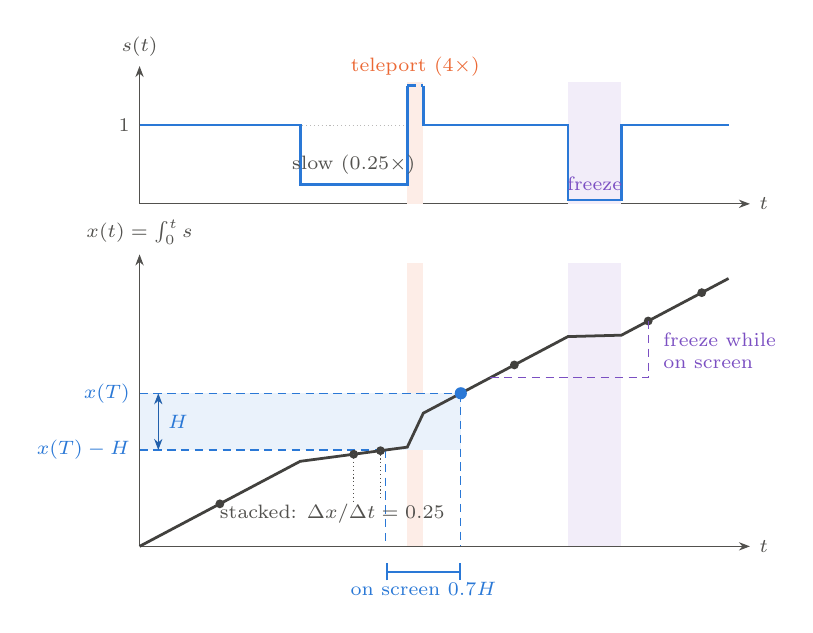
\begin{tikzpicture}[x=0.68cm]
% ---------- top: effective scroll speed s(t) ----------
\def\sy{1.0}
\begin{scope}[yshift=4.35cm]
\draw[->, muted] (0,0) -- (11.4,0) node[lbl, right] {$t$};
\draw[->, muted] (0,0) -- (0,1.75) node[lbl, above] {$s(t)$};
\draw[muted!40, densely dotted] (0,\sy) -- (11,\sy);
\node[lbl, left] at (0,\sy) {1};
\fill[rule!12] (5,0) rectangle (5.3,1.55);
\fill[deep!10] (8,0) rectangle (9,1.55);
\draw[model, line width=1pt] (0,\sy) -- (3,\sy) -- (3,0.25*\sy) -- (5,0.25*\sy) -- (5,1.5) (5.3,1.5) -- (5.3,\sy) -- (8,\sy) -- (8,0.05*\sy) -- (9,0.05*\sy) -- (9,\sy) -- (11,\sy);
\draw[model, line width=1pt, densely dashed] (5,1.5) -- (5.3,1.5);
\node[lbl, above, text=rule] at (5.15,1.5) {teleport ($4\times$)};
\node[lbl, above] at (4.0,0.25) {slow ($0.25\times$)};
\node[lbl, above, text=deep] at (8.5,0.05) {freeze};
\end{scope}
% ---------- bottom: scroll position x(t) ----------
\begin{scope}[y=0.36cm]
\draw[->, muted] (0,0) -- (11.4,0) node[lbl, right] {$t$};
\draw[->, muted] (0,0) -- (0,10.3) node[lbl, above] {$x(t)=\int_0^t s$};
\fill[rule!12] (5,0) rectangle (5.3,10);
\fill[deep!10] (8,0) rectangle (9,10);
% the screen height for the highlighted note (hit at T=6)
\fill[model!10] (0,3.4) rectangle (6,5.4);
\draw[model, densely dashed] (0,5.4) node[lbl, left, text=model] {$x(T)$} -- (6,5.4);
\draw[model, densely dashed] (0,3.4) node[lbl, left, text=model] {$x(T)-H$} -- (4.6,3.4);
\draw[model!80!black, <->] (0.35,3.4) -- node[lbl, right, text=model] {$H$} (0.35,5.4);
\draw[model, densely dashed] (4.6,3.4) -- (4.6,0);
\draw[model, densely dashed] (6,5.4) -- (6,0);
\draw[model, |-|, line width=0.8pt] (4.6,-0.9) -- node[lbl, below, text=model] {on screen $0.7H$} (6,-0.9);
% the curve
\draw[muted!80!black, line width=1pt] (0,0) -- (3,3) -- (5,3.5) -- (5.3,4.7) -- (8,7.4) -- (9,7.45) -- (11,9.45);
% notes
\foreach \T/\X in {1.5/1.5, 4.0/3.25, 4.5/3.375, 6.0/5.4, 7.0/6.4, 9.5/7.95, 10.5/8.95}
  \fill[muted!80!black] (\T,\X) circle (1.6pt);
\fill[model] (6,5.4) circle (2.2pt);
% stacked pair
\draw[muted, densely dotted] (4.0,3.25) -- (4.0,1.6) (4.5,3.375) -- (4.5,1.6);
\node[lbl, align=center] at (3.6,1.15) {stacked: $\Delta x/\Delta t=0.25$};
% the freeze while note 9.5 is visible: its onset
\draw[deep, densely dashed] (6.55,5.95) -- (9.5,5.95);
\draw[deep, densely dashed] (9.5,7.95) -- (9.5,5.95);
\node[lbl, text=deep, align=left, anchor=west] at (9.6,6.9) {freeze while\\on screen};
\end{scope}
\end{tikzpicture}
}
\caption{Reading features. Top: the effective scroll speed $s(t)$ of a chart with a slow section, a teleport and a freeze. Bottom: the scroll position $x(t)$ and the hit times of seven notes (dots). A note hit at $T$ is on screen while $x(T)-x(t)\le H$: the highlighted note appears near the end of the slow section and is visible for only $0.7H$. The two notes in the slow section are drawn a quarter of their time gap apart (stacked), and the freeze happens while the second-to-last note is on screen.}
\label{fig:reading}
\end{figure}

\subsection{MinaCalc ratings}\label{sec:msd}
MinaCalc (Etterna's calculator, version 527) rates a chart on overall difficulty and seven skillsets \citep{minacalc}. We run it at $1.0\times$ on every 4K, 6K and 7K chart, with long notes counted as their heads as in Etterna, and keep the eight ratings and the seven skillset ratings divided by the overall rating, which say what a chart is about independently of how hard it is (15 features).

\subsection{Event tokens}\label{sec:tokens}
For the neural encoders a chart becomes a sequence of \emph{events}, the moments at which at least one note starts or a long note ends (merged within \SI{2}{ms}; \cref{fig:tokens}). Each event carries, per column, three bits: \emph{head} (a note starts), \emph{tail} (an LN is released) and \emph{held} (an LN body passes through the event without starting or ending there). The columns of a $K$-key chart are centred in 10 slots, so 4K and 7K charts share weights, and mirroring the chart reverses the slots. Five continuous values follow: the log gaps to the previous and next event, the gap to the previous event in beats, the log effective scroll speed and the log beat length; then a one-hot snap of the previous gap (1/1, 1/2, 1/4, 1/8, 1/16, 1/3, 1/6, 1/12, other). An event is thus a vector of $10\cdot3+5+9=44$ values; the key count enters the model separately. Events are grouped into 4-second windows by their time from the first event.

\begin{figure*}[t]
\centering
\resizebox{\textwidth}{!}{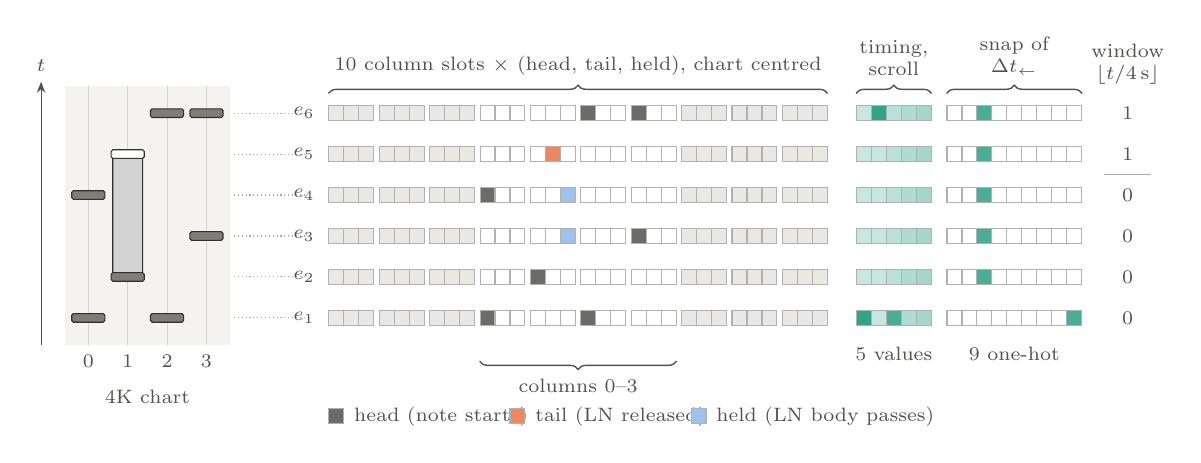
\begin{tikzpicture}[
  tc/.style={draw=muted!45, minimum size=0.19cm, inner sep=0pt},
  brace/.style={decorate, decoration={brace, amplitude=3pt}, draw=muted, line width=0.5pt}]
\def\dy{0.52}
% ---------- the chart ----------
\fill[faint!50] (-0.3,-0.35) rectangle (1.8,{5*\dy+0.35});
\foreach \c in {0,...,3} {\draw[muted!25] ({\c*0.5},-0.35) -- ({\c*0.5},{5*\dy+0.35}); \node[lbl] at ({\c*0.5},-0.55) {\c};}
\draw[lnbody] (0.31,{1*\dy}) rectangle (0.69,{4*\dy});
\foreach \e/\cs in {0/{0,2}, 1/{1}, 2/{3}, 3/{0}, 5/{2,3}} \foreach \c in \cs \node[note] at ({\c*0.5},{\e*\dy}) {};
\node[note, fill=white] at (0.5,{4*\dy}) {};
\node[lbl, align=center] at (0.75,-1.0) {4K chart};
\draw[->, muted] (-0.6,-0.35) -- (-0.6,{5*\dy+0.4}) node[lbl, above] {$t$};
% ---------- event rows ----------
\foreach \e in {0,...,5} {
  \draw[muted!50, densely dotted] (1.85,{\e*\dy}) -- (2.75,{\e*\dy});
  \node[lbl, anchor=east] at (3.0,{\e*\dy}) {$e_{\the\numexpr\e+1\relax}$};
}
% ---------- column slots: 10 x (head, tail, held) ----------
\def\xo{3.15}
\newcommand{\slotx}[2]{\xo+#1*0.64+#2*0.19}
\foreach \e in {0,...,5} \foreach \s in {0,...,9} \foreach \c in {0,1,2} {
  \pgfmathsetmacro{\xx}{\slotx{\s}{\c}}
  \ifnum\s<3 \node[tc, fill=faint] at (\xx,{\e*\dy}) {};
  \else\ifnum\s>6 \node[tc, fill=faint] at (\xx,{\e*\dy}) {};
  \else \node[tc] at (\xx,{\e*\dy}) {}; \fi\fi
}
% ones: event / slot / channel (0 head, 1 tail, 2 held); 4K column c sits in slot c+3
\foreach \e/\s/\c/\col in {0/3/0/muted!85, 0/5/0/muted!85, 1/4/0/muted!85, 2/6/0/muted!85, 2/4/2/model!45, 3/3/0/muted!85, 3/4/2/model!45, 4/4/1/rule!80, 5/5/0/muted!85, 5/6/0/muted!85} {
  \pgfmathsetmacro{\xx}{\slotx{\s}{\c}}
  \node[tc, fill=\col] at (\xx,{\e*\dy}) {};
}
\pgfmathsetmacro{\xa}{\slotx{0}{0}}\pgfmathsetmacro{\xb}{\slotx{9}{2}}
\draw[brace] (\xa-0.1,{5*\dy+0.25}) -- (\xb+0.1,{5*\dy+0.25}) node[lbl, midway, above=3pt, align=center] {10 column slots $\times$ (head, tail, held), chart centred};
\pgfmathsetmacro{\xm}{\slotx{3}{0}}\pgfmathsetmacro{\xn}{\slotx{6}{2}}
\draw[brace, decoration={mirror}] (\xm-0.1,-0.55) -- (\xn+0.1,-0.55) node[lbl, midway, below=3pt] {columns 0--3};
% legend
\pgfmathsetmacro{\xq}{\slotx{0}{0}}
\node[tc, fill=muted!85] (l1) at (\xq,-1.25) {}; \node[lbl, right] at (l1.east) {head (note starts)};
\node[tc, fill=rule!80] (l2) at (\xq+2.3,-1.25) {}; \node[lbl, right] at (l2.east) {tail (LN released)};
\node[tc, fill=model!45] (l3) at (\xq+4.6,-1.25) {}; \node[lbl, right] at (l3.east) {held (LN body passes)};
% ---------- continuous channels ----------
\def\xc{9.85}
\foreach \e/\a/\b/\g in {0/90/25/80, 1/25/25/30, 2/25/25/30, 3/25/25/30, 4/25/25/30, 5/25/90/30} {
  \node[tc, fill=sup!\a] at (\xc,{\e*\dy}) {};
  \node[tc, fill=sup!\b] at (\xc+0.19,{\e*\dy}) {};
  \node[tc, fill=sup!\g] at (\xc+0.38,{\e*\dy}) {};
  \node[tc, fill=sup!35] at (\xc+0.57,{\e*\dy}) {};
  \node[tc, fill=sup!40] at (\xc+0.76,{\e*\dy}) {};
}
\draw[brace] (\xc-0.1,{5*\dy+0.25}) -- (\xc+0.86,{5*\dy+0.25}) node[lbl, midway, above=3pt, align=center] {timing,\\scroll};
\node[lbl, anchor=north] at (\xc+0.38,-0.25) {5 values};
% snap one-hot
\def\xs{11.0}
\foreach \e in {0,...,5} \foreach \k in {0,...,8} \node[tc] at (\xs+\k*0.19,{\e*\dy}) {};
\foreach \e/\k in {0/8, 1/2, 2/2, 3/2, 4/2, 5/2} \node[tc, fill=sup!80] at (\xs+\k*0.19,{\e*\dy}) {};
\draw[brace] (\xs-0.1,{5*\dy+0.25}) -- (\xs+1.62,{5*\dy+0.25}) node[lbl, midway, above=3pt, align=center] {snap of\\$\Delta t_{\leftarrow}$};
\node[lbl, anchor=north] at (\xs+0.76,-0.25) {9 one-hot};
% window index
\def\xw{13.2}
\foreach \e/\w in {0/0, 1/0, 2/0, 3/0, 4/1, 5/1} \node[lbl] at (\xw,{\e*\dy}) {$\w$};
\node[lbl, align=center] at (\xw,{5*\dy+0.62}) {window\\$\lfloor t/4\,\mathrm{s}\rfloor$};
\draw[muted!50] (\xw-0.3,{3.5*\dy}) -- (\xw+0.3,{3.5*\dy});
\end{tikzpicture}
}
\caption{Event tokens. Each moment at which a note starts or a long note ends becomes one event (left: a 4K chart with one long note in column 1). Its vector holds head, tail and held bits for 10 column slots in which the chart's columns are centred (padding in grey), five timing and scroll values (shades) and the snap of the gap to the previous event. The window index groups events into 4-second windows for the encoder of \cref{fig:encoder}.}
\label{fig:tokens}
\end{figure*}

% =====================================================================
\section{Models}\label{sec:models}

\subsection{Rule baselines}\label{sec:rules}
Every learned component has a hand-written counterpart evaluated on identical charts. The slot rule assigns \SV{} if $\min(1,\sigma_{\log s}/0.3)\cdot\min(1,\text{near-note SV rate}/0.5)\ge0.5$, and otherwise the argmax of three LN-share scores: \RC{} $=\mathrm{clip}(1-\rho/0.12)$, \HB{} $=\mathrm{clip}(1-|\rho-0.25|/0.15)$, \LN{} $=\mathrm{clip}((\rho-0.3)/0.3)$. Each tag rule is a product of logistic squashes $\sigma((x-m)/w)$ of the one or two statistics that define the tag (e.g.\ jumpstream $=(1-\sigma_\rho)\,\sigma((\text{jumpstream rows}-0.18)/0.04)$, where $1-\sigma_\rho$ suppresses LN charts); category rules take the maximum over their tags' rules. The thresholds were set by inspecting a few dozen charts before any labels were collected.

\subsection{Slot classifier}\label{sec:slot-model}
The slot model is a histogram gradient-boosting classifier \citep{ke2017lightgbm,pedregosa2011sklearn} on the 71 statistics with 300 iterations, learning rate 0.05, at most 15 leaves, $\ell_2$ regularisation 1.0 and class weights inversely proportional to class frequency (\HB{} and \SV{} are 18\% and 7\% of the data), trained with the multinomial log-loss. Its four probabilities are inputs of the boosted heads; for the tournament charts it was trained on, its out-of-fold probabilities are used.

\subsection{Boosted heads}\label{sec:boosted}
Each task (category or tag) has independent binary heads: boosted classifiers with 200 iterations, learning rate 0.05, 15 leaves, at least 10 samples per leaf and balanced class weights, trained only on charts with a known label. The base input is the concatenation of the statistics, all rule scores and the four slot probabilities, so a head can start from the rule and from the slot model's notion of ``this is an LN chart''. The \emph{boosted component} of the ensemble averages five heads per task, which differ in inputs and labels: base, base + windows, and base + windows + transitions on strict labels, and base + windows and base + windows + transitions on strict and relaxed labels (relaxed pairs at weight $\tfrac12$). For the five \SV{} heads (Reading, Memo and the three \utag{sliders/*} tags) the boosted component is instead a single relaxed-label head on base + windows + transitions + reading + MinaCalc features. The reading features describe scroll speed only, and for the other tasks they would add 37 inputs that carry no signal; we use them where they apply (\cref{sec:res-reading}).

\subsection{Per-fold teachers and targets}\label{sec:teachers}
The neural models learn from the unlabelled majority of the corpus through \emph{teachers}, models of the previous family whose predictions serve as soft targets where a label is missing (\cref{fig:protocol}). For fold $k$, every teacher is trained on folds $\neq k$ and predicts every chart, so its predictions are out-of-sample for fold $k$, and the students of fold $k$ read them only on non-test charts. The chain is:
\begin{enumerate}\setlength\itemsep{1pt}
\item two boosted teachers: the mean of the relaxed-label heads on base + windows and on base + windows + transitions, and the relaxed-label head with reading and MinaCalc features;
\item the MLP student (\cref{sec:mlp}), distilled from the mean of the two boosted teachers;
\item the deep teacher $T_k$, the mean of the two boosted teachers and the MLP student, from which the event encoders are distilled.
\end{enumerate}
For every chart and task, a student's target is the first that exists of the strict label (weight 1), the relaxed label (weight $\tfrac12$) and the teacher's probability (weight 1). The students' binary losses are weighted cross-entropies with a positive weight $\min(10,\max(1,\sqrt{n_-/n_+}))$ per task, from the strict training labels.

\begin{figure*}[t]
\centering
\resizebox{\textwidth}{!}{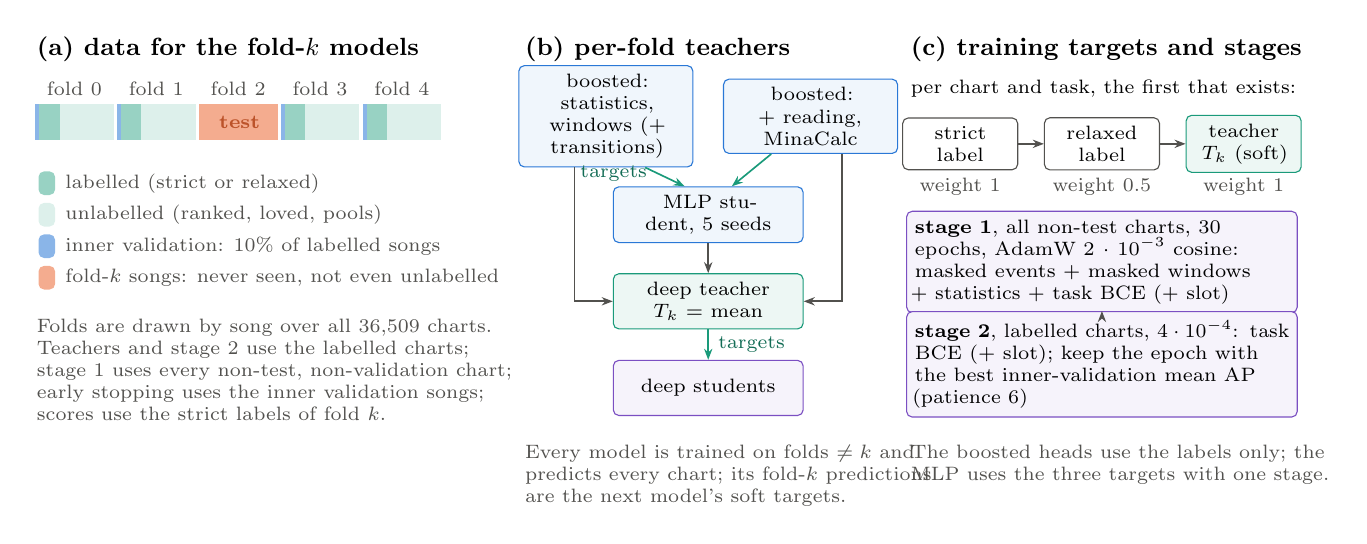
\begin{tikzpicture}[
  mdl/.style={box, draw=model, fill=model!7, minimum height=0.7cm},
  dmdl/.style={box, draw=deep, fill=deep!7, minimum height=0.7cm},
  tch/.style={box, draw=sup, fill=sup!8, minimum height=0.6cm},
  sarr/.style={arr, draw=sup}]
% ================= (a) folds =================
\begin{scope}
\node[font=\small\bfseries, anchor=west] at (-0.1,3.05) {(a) data for the fold-$k$ models};
\def\W{1.04}
\foreach \f in {0,...,4} {
  \pgfmathsetmacro{\xa}{\f*\W}
  \ifnum\f=2
    \fill[rule!55] (\xa,1.9) rectangle (\xa+\W-0.04,2.35);
  \else
    \fill[sup!45] (\xa,1.9) rectangle (\xa+\W*0.3,2.35);
    \fill[sup!15] (\xa+\W*0.3,1.9) rectangle (\xa+\W-0.04,2.35);
    \fill[model!55] (\xa,1.9) rectangle (\xa+\W*0.05,2.35);
  \fi
  \node[lbl] at (\xa+\W/2-0.02,2.55) {fold \f};
}
\node[lbl, text=rule!80!black, font=\scriptsize\bfseries] at (2.6,2.12) {test};
\node[tch, minimum height=0.3cm, fill=sup!45, draw=none] (k1) at (0.15,1.35) {}; \node[lbl, right] at (k1.east) {labelled (strict or relaxed)};
\node[tch, minimum height=0.3cm, fill=sup!15, draw=none] (k2) at (0.15,0.95) {}; \node[lbl, right] at (k2.east) {unlabelled (ranked, loved, pools)};
\node[tch, minimum height=0.3cm, fill=model!55, draw=none] (k3) at (0.15,0.55) {}; \node[lbl, right] at (k3.east) {inner validation: 10\% of labelled songs};
\node[tch, minimum height=0.3cm, fill=rule!55, draw=none] (k4) at (0.15,0.15) {}; \node[lbl, right] at (k4.east) {fold-$k$ songs: never seen, not even unlabelled};
\node[lbl, align=left, anchor=north west] at (-0.1,-0.25) {Folds are drawn by song over all \nCharts{} charts.\\Teachers and stage 2 use the labelled charts;\\stage 1 uses every non-test, non-validation chart;\\early stopping uses the inner validation songs;\\scores use the strict labels of fold $k$.};
\end{scope}
% ================= (b) teacher chain =================
\begin{scope}[xshift=6.3cm]
\node[font=\small\bfseries, anchor=west] at (-0.2,3.05) {(b) per-fold teachers};
\node[mdl, text width=2.0cm, font=\scriptsize] (b1) at (0.95,2.2) {boosted: statistics,\\windows (+ transitions)};
\node[mdl, text width=2.0cm, font=\scriptsize] (b2) at (3.55,2.2) {boosted: + reading,\\MinaCalc};
\node[mdl, text width=2.2cm, font=\scriptsize] (mlp) at (2.25,0.95) {MLP student, 5 seeds};
\node[tch, text width=2.2cm, font=\scriptsize] (t) at (2.25,-0.15) {deep teacher $T_k$ = mean};
\node[dmdl, text width=2.2cm, font=\scriptsize] (deep) at (2.25,-1.25) {deep students};
\draw[sarr] (b1.south) ++(0.5,0) -- node[lbl, left, text=sup!70!black, pos=0.3] {targets} ([xshift=-3mm]mlp.north);
\draw[sarr] (b2.south) ++(-0.5,0) -- ([xshift=3mm]mlp.north);
\draw[arr] (b1.south) ++(-0.4,0) |- (t.west);
\draw[arr] (b2.south) ++(0.4,0) |- (t.east);
\draw[arr] (mlp) -- (t);
\draw[sarr] (t) -- node[lbl, right, text=sup!70!black] {targets} (deep);
\node[lbl, align=left, anchor=north west] at (-0.2,-1.85) {Every model is trained on folds $\neq k$ and\\predicts every chart; its fold-$k$ predictions\\are the next model's soft targets.};
\end{scope}
% ================= (c) targets and stages =================
\begin{scope}[xshift=11.2cm]
\node[font=\small\bfseries, anchor=west] at (-0.2,3.05) {(c) training targets and stages};
\node[lbl, anchor=west, text=black] at (-0.2,2.55) {per chart and task, the first that exists:};
\node[box, text width=1.25cm, font=\scriptsize] (s1) at (0.55,1.85) {strict label};
\node[box, text width=1.25cm, font=\scriptsize] (s2) at (2.35,1.85) {relaxed label};
\node[tch, text width=1.25cm, font=\scriptsize] (s3) at (4.15,1.85) {teacher $T_k$ (soft)};
\draw[arr] (s1) -- (s2); \draw[arr] (s2) -- (s3);
\node[lbl] at (0.55,1.3) {weight 1};
\node[lbl] at (2.35,1.3) {weight 0.5};
\node[lbl] at (4.15,1.3) {weight 1};
\node[dmdl, text width=4.75cm, font=\scriptsize, align=left] (st1) at (2.35,0.35) {\textbf{stage 1}, all non-test charts, 30 epochs, AdamW $2\cdot10^{-3}$ cosine: masked events + masked windows + statistics + task BCE (+ slot)};
\node[dmdl, text width=4.75cm, font=\scriptsize, align=left] (st2) at (2.35,-0.95) {\textbf{stage 2}, labelled charts, $4\cdot10^{-4}$: task BCE (+ slot); keep the epoch with the best inner-validation mean AP (patience 6)};
\draw[arr] (st1) -- (st2);
\node[lbl, align=left, anchor=north west] at (-0.2,-1.85) {The boosted heads use the labels only; the\\MLP uses the three targets with one stage.};
\end{scope}
\end{tikzpicture}
}
\caption{Training protocol for fold $k$. (a) Folds are drawn by song over the whole corpus, so fold-$k$ songs are excluded from every stage of every fold-$k$ model, including pretraining on unlabelled charts. (b) Each model family is distilled from the per-fold predictions of the previous ones. (c) Targets fall back from strict labels to relaxed labels to the teacher; the event encoders are trained in two stages.}
\label{fig:protocol}
\end{figure*}

\subsection{MLP student}\label{sec:mlp}
One multi-task network predicts all 31 tasks from the boosted heads' feature vector without rule scores and slot probabilities: statistics and window statistics (signed log), row transitions, reading features and MinaCalc ratings, z-scored on the fold's training charts. It has two hidden layers of 512 and 256 GELU units, dropout 0.1 on the input and 0.3 on the hidden layers, and is trained with AdamW \citep{loshchilov2019adamw} (learning rate $10^{-3}$, weight decay 0.05, batches of 256) on every non-test chart with the targets of \cref{sec:teachers}. Training stops when the mean AP on the inner-validation songs (over tasks with at least five validation positives) has not improved for 8 epochs, and the best epoch is kept. The component averages five seeds.

\subsection{Deep event encoder}\label{sec:deep}
\paragraph{Architecture.} The encoder reads the event tokens of \cref{sec:tokens} hierarchically (\cref{fig:encoder}). A linear layer maps each event to 64 channels and adds an embedding of the key count. Six residual blocks, each a GroupNorm \citep{wu2018groupnorm}, a convolution of width 3 with dilation $2^{i}$ ($i=0,\dots,5$) and a gated linear unit \citep{dauphin2017glu}, give every event a context of 127 events, enough for the patterns of \cref{fig:features}. Events are then pooled into 4-second windows by concatenating their mean and maximum, followed by a linear layer, GELU and LayerNorm. A learned position embedding is added to the window tokens, and a two-layer pre-norm transformer \citep{vaswani2017attention} with 4 heads relates the windows of the whole chart. Each task $\tau$ reads the window embeddings $h_w$ with its own gated attention \citep{ilse2018attention},
\begin{align}
a_{\tau w}&=\operatorname*{softmax}_w\, u_\tau^{\!\top}\!\big(\tanh(V_\tau h_w)\odot\sigma(U_\tau h_w)\big),\\
z_\tau&=\textstyle\sum_w a_{\tau w}h_w,
\end{align}
and a linear classifier on $z_\tau$ gives the logit. The attention weights say in which windows a skillset was found. A four-way slot head reads the mean window embedding.

\paragraph{Stage 1: pretraining and distillation.} On every non-test, non-validation chart of the fold (about \num{26000}), the encoder is trained for up to 30 epochs on the sum of four objectives:
\begin{itemize}\setlength\itemsep{1pt}
\item \emph{masked events}: 15\% of the events are replaced by a learned vector after the input layer, and from their encoded features the model predicts their head and tail bits per column and their log gap to the previous event (pattern grammar);
\item \emph{masked windows}: 15\% of the window tokens are replaced by a learned vector before the transformer, and the model predicts 17 summary statistics of each masked window (log counts of events and notes; shares of chords, jacks, releases and held columns; mean gap and scroll speed; snap distribution) from the surrounding windows (structure);
\item \emph{statistics}: from the mean and maximum of the window embeddings, the model regresses the 260 chart and window statistics (signed log, z-scored, smooth $\ell_1$), which are free targets on every chart;
\item \emph{tasks}: the weighted cross-entropy against the targets of \cref{sec:teachers}, plus half the cross-entropy of the slot head on tournament charts.
\end{itemize}
Optimisation uses AdamW with learning rate $2\cdot10^{-3}$, weight decay 0.02, linear warm-up over the first 1/30 of the steps and cosine decay, gradient clipping at 1, and batches of charts of similar length with at most \num{64000} padded events. Training charts are cropped to a random span of \num{4000} events and mirrored with probability $\tfrac12$.

\paragraph{Stage 2: fine-tuning.} The self-supervised and statistics losses are dropped, and the model is fine-tuned on the charts that have a strict or relaxed label (teacher targets fill their unknown tasks) at learning rate $4\cdot10^{-4}$ for up to 25 epochs. After each epoch of both stages the mean AP on the inner-validation songs is computed; a stage stops after 6 epochs without improvement and keeps its best state. Test charts are read whole (up to \num{12000} events), and the prediction is the mean over the chart and its mirror image.

\paragraph{Wide path.} The second deep component adds the boosted heads' feature vector (statistics, window statistics, transitions, reading and MinaCalc features, z-scored) through an MLP ($128\to64\to35$ units) whose logits are added to the attention heads' task and slot logits, as in wide-and-deep models \citep{cheng2016wide}. During training the whole wide path is switched off for a random half of the charts in each batch, so that the event encoder still has to classify on its own and the two paths do not co-adapt. The plain component averages \nPlain{} seeds and the wide component \nWide{}.

\begin{figure*}[t]
\centering
\resizebox{\textwidth}{!}{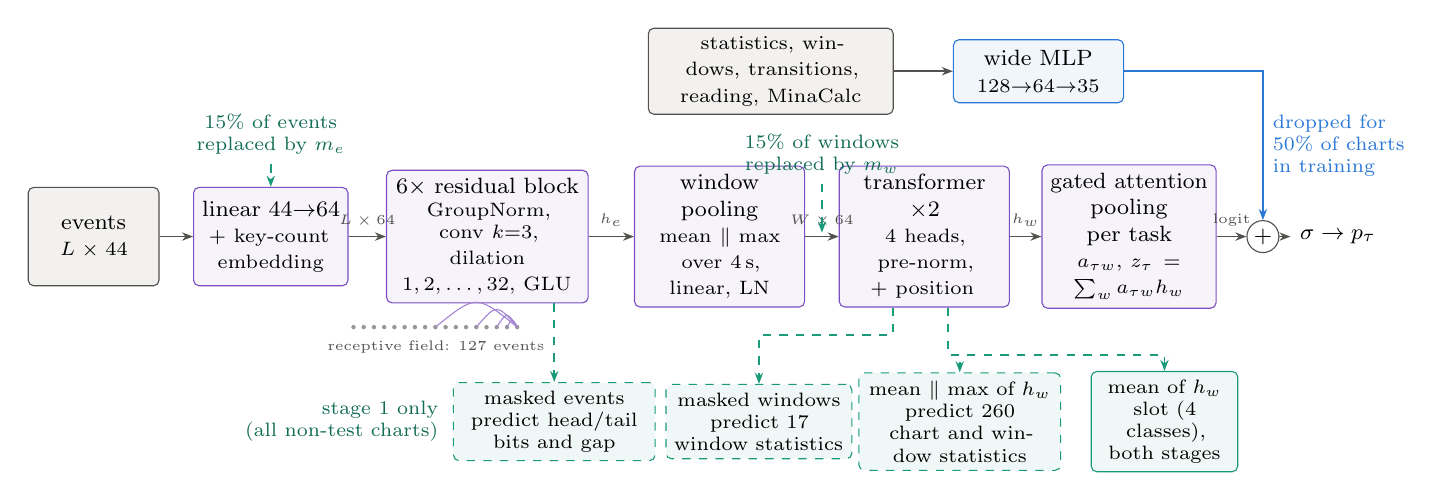
\begin{tikzpicture}[
  blk/.style={box, draw=deep, fill=deep!7, minimum height=1.25cm},
  io/.style={box, fill=faint!60, minimum height=1.25cm},
  aux/.style={box, draw=sup, fill=sup!7, dashed, minimum height=0.8cm, font=\scriptsize},
  wd/.style={box, draw=model, fill=model!7, minimum height=0.8cm},
  dim/.style={lbl, font=\tiny, text=muted},
  sarr/.style={arr, draw=sup, dashed}]
% ---------- main path ----------
\node[io, text width=1.45cm] (x) at (0,0) {events\\{\scriptsize $L\times44$}};
\node[blk, text width=1.75cm] (emb) at (2.25,0) {linear $44{\to}64$\\{\scriptsize + key-count embedding}};
\node[blk, text width=2.35cm] (conv) at (5.0,0) {$6\times$ residual block\\{\scriptsize GroupNorm, conv $k{=}3$,\\dilation $1,2,\dots,32$, GLU}};
\node[blk, text width=1.95cm] (pool) at (7.95,0) {window pooling\\{\scriptsize mean $\Vert$ max over 4\,s, linear, LN}};
\node[blk, text width=1.95cm] (tf) at (10.55,0) {transformer $\times2$\\{\scriptsize 4 heads, pre-norm, + position}};
\node[blk, text width=2.0cm] (mil) at (13.15,0) {gated attention\\pooling per task\\{\scriptsize $a_{\tau w}$, $z_\tau=\sum_w a_{\tau w}h_w$}};
\node[circle, draw=muted, inner sep=1pt, font=\footnotesize] (plus) at (14.85,0) {$+$};
\node[lbl, right, font=\footnotesize, text=black] (out) at (15.2,0) {$\sigma\to p_\tau$};
\draw[arr] (x) -- (emb);
\draw[arr] (emb) -- node[dim, above] {$L\times64$} (conv);
\draw[arr] (conv) -- node[dim, above] {$h_e$} (pool);
\draw[arr] (pool) -- node[dim, above] {$W\times64$} (tf);
\draw[arr] (tf) -- node[dim, above] {$h_w$} (mil);
\draw[arr] (mil) -- node[dim, above] {logit} (plus);
\draw[arr] (plus) -- (out);
% receptive field inset under the conv stack
\begin{scope}[shift={(3.3,-1.15)}]
\foreach \i in {0,...,16} \fill[muted!60] (\i*0.13,0) circle (0.8pt);
\foreach \d/\h in {1/0.12, 2/0.2, 4/0.3, 8/0.42} {
  \draw[deep!70, line width=0.4pt] ({(16-\d)*0.13},0) .. controls ({(16-\d*0.5)*0.13},\h) .. ({16*0.13},0);
}
\node[dim, anchor=north, align=center] at (1.05,-0.05) {receptive field: 127 events};
\end{scope}
% ---------- wide path ----------
\node[io, text width=2.9cm, minimum height=0.8cm] (wfeat) at (8.6,2.1) {{\scriptsize statistics, windows, transitions, reading, MinaCalc}};
\node[wd, text width=1.95cm] (wmlp) at (12.0,2.1) {wide MLP\\{\scriptsize $128{\to}64{\to}35$}};
\draw[arr] (wfeat) -- (wmlp);
\draw[arr, draw=model] (wmlp.east) -| node[lbl, right, pos=0.75, text=model, align=left] {dropped for\\50\% of charts\\in training} (plus.north);
% ---------- stage-1 objectives ----------
\node[aux, text width=2.35cm] (mev) at (5.85,-2.35) {masked events\\predict head/tail bits and gap};
\node[aux, text width=2.15cm] (mwin) at (8.45,-2.35) {masked windows\\predict 17 window statistics};
\node[aux, text width=2.35cm] (stats) at (11.0,-2.35) {mean $\Vert$ max of $h_w$\\predict 260 chart and window statistics};
\node[aux, solid, text width=1.65cm] (slot) at (13.6,-2.35) {mean of $h_w$\\slot (4 classes), both stages};
\draw[sarr] (conv.south -| mev.north) -- (mev.north);
\draw[sarr] (tf.south) ++(-0.4,0) -- ++(0,-0.35) -| (mwin.north);
\draw[sarr] (tf.south) ++(0.3,0) -- ++(0,-0.6) -| (stats.north);
\draw[sarr] (tf.south) ++(0.3,0) -- ++(0,-0.6) -| (slot.north);
% masking inputs
\node[lbl, text=sup!70!black, align=center] (m1) at (2.25,1.3) {15\% of events\\replaced by $m_e$};
\draw[sarr] (m1) -- (emb.north);
\node[lbl, text=sup!70!black, align=center] (m2) at (9.25,1.05) {15\% of windows\\replaced by $m_w$};
\draw[sarr] (m2.south) -- (9.25,0.05);
\node[lbl, text=sup!70!black, anchor=east, align=right] at (4.5,-2.35) {stage 1 only\\(all non-test charts)};
\end{tikzpicture}
}
\caption{The event encoder. Dilated gated convolutions read local patterns from the event tokens, events are pooled into 4-second windows, a transformer relates the windows of the whole chart, and one gated attention pool per task selects the windows that carry the skillset. The wide path (blue) adds a logit from the chart-level features. The dashed heads are trained only in stage 1, on every non-test chart: masked event and masked window prediction, and regression of the chart and window statistics.}
\label{fig:encoder}
\end{figure*}

\subsection{Ensemble}\label{sec:ensemble}
The final prediction for each task is the unweighted mean of the probabilities of the four components (boosted, MLP, deep, wide \& deep), each itself the mean of its runs. Nothing in the combination is fitted, so the combination cannot overfit the evaluation folds.

\subsection{Reported output}
For a new chart the system reports its argmax slot, the categories of that slot whose score exceeds the head's threshold (for \HB, the Rice and LN categories), any category of another slot whose score exceeds $\max(\text{threshold},0.8)$, Mixed Rice by the rule of \cref{sec:categories}, a TB flag, and timestamps of the densest jack, stream, LN and \SV{} sections. Thresholds maximise F1 on the out-of-fold predictions.

% =====================================================================
\section{Experimental setup}\label{sec:setup}
\paragraph{Slots.} The slot model is evaluated by 5-fold stratified cross-validation grouped by song on the \num{4029} slot-labelled charts. We report accuracy and macro-F1 with a cluster bootstrap over songs \citep{efron1993bootstrap} (\num{1000} replicates).

\paragraph{Categories and tags.} All models use the five song folds of \cref{sec:corpus}. Inside the training folds, 10\% of the songs that have a labelled chart are held out as \emph{inner validation} for early stopping; the test fold is never used for any choice within a run. Each task is scored by average precision (AP) on the pooled out-of-fold predictions of its strictly labelled charts, which is threshold-free and suited to rare positives \citep{davis2006pr,saito2015pr}, and each benchmark by the mean AP over its tasks (11 categories, 20 tags). The reference is the boosted head on base + windows with strict labels (\emph{gbm+win}), the strongest single head of the boosted family. Differences are given with a paired cluster bootstrap over songs: songs are resampled with replacement \nBoot{} times, and on each resample the AP of every task is recomputed for both models on the same charts. The neural models were trained on one RTX 2060 SUPER (8\,GB), about 1.5 hours for the five folds of one deep run; the boosted heads on four CPU cores.

% =====================================================================
\section{Results}\label{sec:results}

\subsection{Tournament slots}\label{sec:res-slots}
\begin{table*}[t]
\centering\small
\caption{Slot classification on 4{,}029 tournament charts (5-fold CV grouped by song). Brackets: 95\% cluster-bootstrap intervals over songs. The accuracy gain is 9.6 points [8.6, 10.6].}
\label{tab:slots}
\begin{tabular}{lcccccccc}
\toprule
& & & \multicolumn{4}{c}{F1 per slot} & \multicolumn{2}{c}{accuracy by keys} \\
\cmidrule(lr){4-7}\cmidrule(lr){8-9}
Method & Accuracy (\%) & Macro-F1 & \RC & \LN & \HB & \SV & 4K & 7K \\
\midrule
Rule baseline & 88.5 [87.5, 89.4] & 0.844 [0.831, 0.856] & 0.995 & 0.843 & 0.566 & 0.970 & 88.6 & 89.0 \\
Gradient boosting & 98.1 [97.7, 98.5] & 0.978 [0.973, 0.983] & 0.994 & 0.977 & 0.951 & 0.991 & 98.1 & 98.1 \\
\bottomrule
\end{tabular}
\end{table*}

The learned slot classifier reaches 98.1\% accuracy and 0.978 macro-F1, against 88.5\% and 0.844 for the slotting rules; the 9.6-point gain has a 95\% interval of $[8.6, 10.6]$, and the improvement holds for each key mode (\cref{tab:slots}). \Cref{fig:confusion} locates the difference. Rice and scroll-speed charts are easy for both methods. The rules mislabel 427 of 738 hybrids (58\%) as long-note charts, because tournament hybrids are far more LN-heavy than the rule's notion of ``some LNs'': their median LN share is 0.38, and a third of them exceed the point (0.37) at which the rule prefers \LN{} (\cref{fig:lnshare}). The learned model raises hybrid F1 from 0.566 to 0.951. Its 77 remaining errors are mostly the same boundary in both directions (median LN share 0.53) and cluster in a few tournaments, partly because the normaliser labels every o!mLN chart \LN{} although some of its pools contain hybrids. Two quantities nearly determine the slot: LN share alone gives 90.0\% accuracy, and adding the nine scroll-speed statistics gives 96.7\%. A random forest or a logistic regression on the same 71 statistics comes within 0.2 points of boosting, so the gain comes from placing the boundaries where organisers place them rather than from the model class.

\begin{figure}[t]
\centering
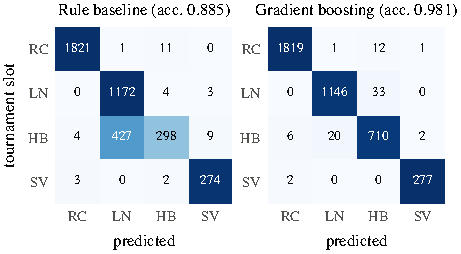
\includegraphics[width=\columnwidth]{fig/confusion.pdf}
\caption{Slot confusion matrices (counts; shading is row-normalised). Nearly all rule errors are hybrids labelled LN.}
\label{fig:confusion}
\end{figure}

\begin{figure}[t]
\centering
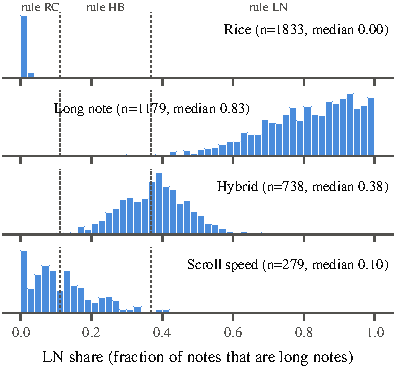
\includegraphics[width=\columnwidth]{fig/ln_share.pdf}
\caption{LN share of tournament charts by slot. Dashed lines mark where the rule's \RC/\HB{} and \HB/\LN{} scores cross. Hybrids span 0.1 to 0.7 and overlap the LN distribution.}
\label{fig:lnshare}
\end{figure}

\subsection{Categories and user tags}\label{sec:res-main}
\begin{table*}[t]
\centering\small
\caption{Reviewer categories. Average precision on the strict out-of-fold labels (song-grouped 5-fold CV over all charts). pos./known: positive and labelled charts. gbm+win is the reference boosted head; the four components are averaged into the ensemble. Bold: best learned model. $^\dagger$\,\SV{} heads, for which the boosted component uses the reading and MinaCalc features.}
\label{tab:v2-cats}
\begin{tabular}{lrrccccccc}
\toprule
& & & & & \multicolumn{4}{c}{components} & \\ \cmidrule(lr){6-9}
Task & pos. & known & rule & gbm+win & boosted & MLP & deep & wide\,\&\,deep & ensemble \\
\midrule
Chordjack & 1057 & 3495 & 0.772 & 0.841 & 0.851 & 0.843 & 0.844 & 0.852 & \textbf{0.856} \\
Streams & 958 & 3327 & 0.479 & 0.585 & 0.610 & 0.624 & 0.626 & 0.633 & \textbf{0.635} \\
Jumpstream/Handstream & 1460 & 3612 & 0.679 & 0.817 & 0.827 & 0.837 & 0.839 & \textbf{0.844} & 0.843 \\
Technical & 723 & 3359 & 0.607 & 0.737 & 0.752 & 0.766 & 0.764 & 0.772 & \textbf{0.776} \\
Stamina & 1229 & 3384 & 0.614 & 0.779 & 0.785 & 0.785 & 0.782 & 0.790 & \textbf{0.793} \\
Release & 342 & 3349 & 0.368 & 0.718 & 0.732 & 0.717 & 0.740 & 0.733 & \textbf{0.741} \\
Coordination & 744 & 3556 & 0.543 & 0.752 & 0.765 & 0.772 & 0.777 & 0.772 & \textbf{0.780} \\
Density/Inverse & 486 & 3376 & 0.657 & 0.735 & 0.756 & 0.747 & 0.770 & 0.769 & \textbf{0.773} \\
Reading$^\dagger$ & 485 & 3449 & 0.798 & 0.895 & \textbf{0.915} & 0.905 & 0.874 & 0.902 & 0.914 \\
Memo$^\dagger$ & 43 & 3241 & 0.289 & 0.267 & 0.438 & 0.480 & 0.497 & 0.528 & \textbf{0.531} \\
TB & 585 & 7644 & 0.402 & 0.787 & 0.803 & 0.737 & 0.750 & 0.782 & \textbf{0.805} \\
\midrule
Mean & & & 0.564 & 0.719 & 0.749 & 0.747 & 0.751 & 0.762 & \textbf{0.768} \\
\bottomrule
\end{tabular}
\end{table*}

\begin{table*}[t]
\centering\small
\caption{User tags. Average precision on the strict out-of-fold labels (song-grouped 5-fold CV over all charts). pos./known: positive and labelled charts. gbm+win is the reference boosted head; the four components are averaged into the ensemble. Bold: best learned model. $^\dagger$\,\SV{} heads, for which the boosted component uses the reading and MinaCalc features.}
\label{tab:v2-tags}
\begin{tabular}{lrrccccccc}
\toprule
& & & & & \multicolumn{4}{c}{components} & \\ \cmidrule(lr){6-9}
Task & pos. & known & rule & gbm+win & boosted & MLP & deep & wide\,\&\,deep & ensemble \\
\midrule
\utag{style/jumpstream} & 945 & 3276 & 0.538 & 0.718 & 0.736 & 0.735 & 0.742 & 0.747 & \textbf{0.748} \\
\utag{style/handstream} & 298 & 3199 & 0.179 & 0.503 & 0.521 & 0.534 & 0.529 & 0.536 & \textbf{0.545} \\
\utag{style/chordstream} & 479 & 3324 & 0.481 & 0.561 & 0.581 & 0.592 & 0.586 & 0.591 & \textbf{0.596} \\
\utag{style/quadstream} & 36 & 3218 & 0.091 & 0.077 & 0.115 & 0.147 & \textbf{0.164} & 0.158 & 0.153 \\
\utag{style/chordjack} & 1020 & 3420 & 0.804 & 0.850 & 0.860 & 0.863 & 0.867 & 0.865 & \textbf{0.868} \\
\utag{skillset/speedjack} & 743 & 3297 & 0.531 & 0.625 & 0.651 & 0.632 & 0.657 & 0.661 & \textbf{0.672} \\
\utag{style/longjack} & 214 & 3211 & 0.243 & 0.477 & 0.494 & 0.502 & 0.495 & 0.523 & \textbf{0.526} \\
\utag{skillset/wristjack} & 310 & 3200 & 0.377 & 0.368 & 0.385 & 0.408 & 0.401 & 0.404 & \textbf{0.410} \\
\utag{skillset/streams} & 958 & 3327 & 0.479 & 0.585 & 0.610 & 0.624 & 0.623 & 0.631 & \textbf{0.633} \\
\utag{streams/speed} & 675 & 3261 & 0.263 & 0.522 & 0.547 & 0.549 & 0.542 & 0.554 & \textbf{0.564} \\
\utag{streams/stamina} & 1228 & 3294 & 0.622 & 0.794 & 0.802 & 0.800 & 0.797 & 0.802 & \textbf{0.808} \\
\utag{skillset/tech} & 684 & 3352 & 0.566 & 0.715 & 0.732 & 0.749 & 0.748 & 0.757 & \textbf{0.760} \\
\utag{style/LN density} & 324 & 3269 & 0.630 & 0.613 & 0.639 & 0.654 & \textbf{0.665} & \textbf{0.665} & 0.663 \\
\utag{style/LN release} & 342 & 3349 & 0.368 & 0.718 & 0.732 & 0.717 & \textbf{0.744} & 0.733 & 0.742 \\
\utag{style/LN coordination} & 722 & 3489 & 0.584 & 0.750 & 0.769 & 0.781 & \textbf{0.790} & 0.783 & 0.789 \\
\utag{gimmick/LN inverse} & 209 & 3247 & 0.384 & 0.450 & 0.490 & 0.530 & \textbf{0.541} & 0.534 & 0.532 \\
\utag{style/generic hybrid} & 421 & 3348 & 0.316 & 0.582 & 0.616 & 0.627 & 0.625 & 0.622 & \textbf{0.638} \\
\utag{sliders/complex sv}$^\dagger$ & 247 & 3304 & 0.894 & 0.909 & 0.919 & \textbf{0.925} & 0.900 & 0.907 & 0.921 \\
\utag{sliders/low sv}$^\dagger$ & 183 & 3268 & 0.312 & 0.533 & 0.643 & 0.641 & 0.610 & 0.643 & \textbf{0.663} \\
\utag{sliders/high sv}$^\dagger$ & 141 & 3256 & 0.387 & 0.418 & 0.470 & \textbf{0.482} & 0.468 & 0.457 & \textbf{0.482} \\
\midrule
Mean & & & 0.452 & 0.588 & 0.616 & 0.625 & 0.625 & 0.629 & \textbf{0.636} \\
\bottomrule
\end{tabular}
\end{table*}

\Cref{tab:v2-cats,tab:v2-tags} give the AP of every task, and \cref{fig:pertask} shows them against the rules and the reference. The ensemble reaches a mean AP of \catEns{} on the categories and \tagEns{} on the tags, against \catBase{} and \tagBase{} for gbm+win and \catRule{} and \tagRule{} for the rules. The gain over gbm+win is $\catGain$ on the categories, with a 95\% song-bootstrap interval of $[\catLo, \catHi]$, and $\tagGain$ on the tags, $[\tagLo, \tagHi]$. The ensemble is better than gbm+win on \catBeatsBase{} of 11 categories and \tagBeatsBase{} of 20 tags.

The gains are largest where the reference lacked information. Memo rises from \apMemoBase{} to \apMemoEns{} and \utag{sliders/low sv} from 0.53 to 0.66, through the reading features (\cref{sec:res-reading}). Skillsets defined by transitions or by sections gain 0.04 to 0.08: LN inverse ($+0.08$); generic hybrid, longjack, speedjack, tech, stream speed and handstream ($+0.04$ to $+0.06$); and Streams, Technical and Density/Inverse among the categories ($+0.04$ to $+0.05$). Skillsets that one statistic already captures, such as chordjack (0.87) or complex SV (0.92), gain least. The weakest tasks are the rarest: \utag{style/quadstream} has 36 positives and stays at 0.15 AP, and wristjack reaches 0.41.

\begin{figure}[t]
\centering
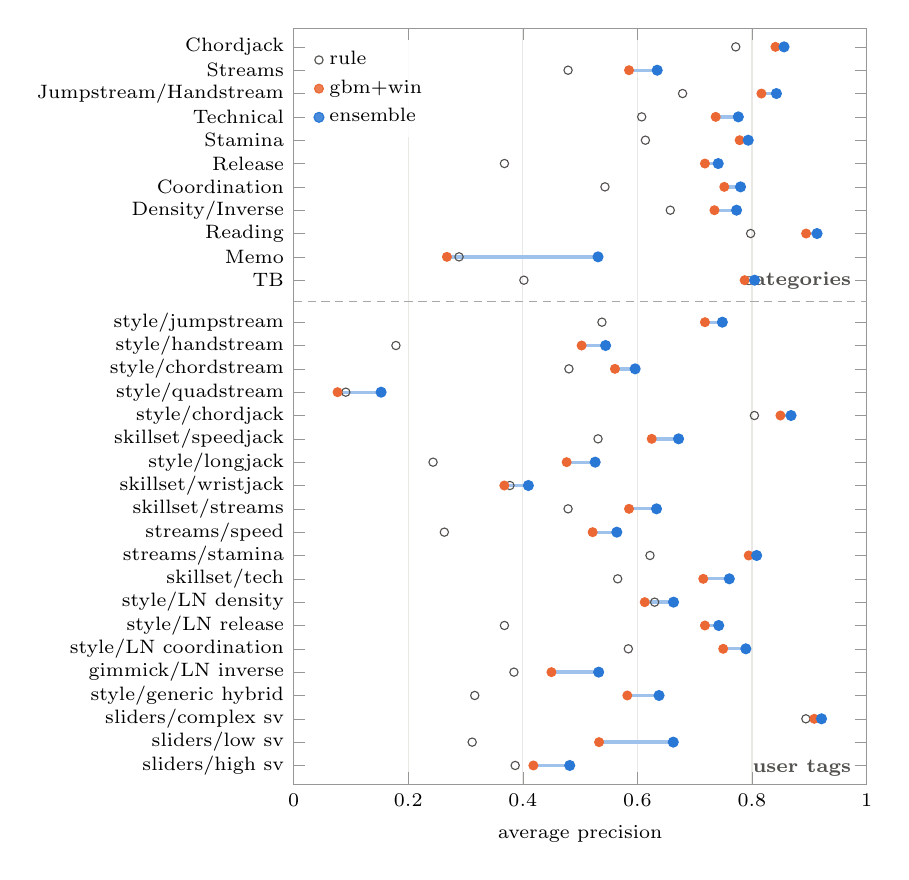
\begin{tikzpicture}
\begin{axis}[scale only axis, width=0.6\columnwidth, height=9.6cm, xmin=0, xmax=1, ymin=-0.8, ymax=31.6,
  ytick={30.8,29.8,28.8,27.8,26.8,25.8,24.8,23.8,22.8,21.8,20.8,19.0,18.0,17.0,16.0,15.0,14.0,13.0,12.0,11.0,10.0,9.0,8.0,7.0,6.0,5.0,4.0,3.0,2.0,1.0,0.0},
  yticklabels={{Chordjack},{Streams},{Jumpstream/Handstream},{Technical},{Stamina},{Release},{Coordination},{Density/Inverse},{Reading},{Memo},{TB},{style/jumpstream},{style/handstream},{style/chordstream},{style/quadstream},{style/chordjack},{skillset/speedjack},{style/longjack},{skillset/wristjack},{skillset/streams},{streams/speed},{streams/stamina},{skillset/tech},{style/LN density},{style/LN release},{style/LN coordination},{gimmick/LN inverse},{style/generic hybrid},{sliders/complex sv},{sliders/low sv},{sliders/high sv}},
  yticklabel style={font=\scriptsize}, xticklabel style={font=\scriptsize}, xlabel={average precision}, xlabel style={font=\scriptsize}, xmajorgrids, grid style={faint}, axis line style={muted!60}, tick style={muted!60},
  legend style={font=\scriptsize, at={(0.02,0.985)}, anchor=north west, draw=none, fill=white, fill opacity=0.85, text opacity=1}, legend cell align=left]
\draw[model!45, line width=1.2pt] (axis cs:0.8410,30.8) -- (axis cs:0.8560,30.8);
\draw[model!45, line width=1.2pt] (axis cs:0.5854,29.8) -- (axis cs:0.6346,29.8);
\draw[model!45, line width=1.2pt] (axis cs:0.8165,28.8) -- (axis cs:0.8427,28.8);
\draw[model!45, line width=1.2pt] (axis cs:0.7367,27.8) -- (axis cs:0.7762,27.8);
\draw[model!45, line width=1.2pt] (axis cs:0.7785,26.8) -- (axis cs:0.7935,26.8);
\draw[model!45, line width=1.2pt] (axis cs:0.7179,25.8) -- (axis cs:0.7411,25.8);
\draw[model!45, line width=1.2pt] (axis cs:0.7517,24.8) -- (axis cs:0.7801,24.8);
\draw[model!45, line width=1.2pt] (axis cs:0.7345,23.8) -- (axis cs:0.7731,23.8);
\draw[model!45, line width=1.2pt] (axis cs:0.8945,22.8) -- (axis cs:0.9136,22.8);
\draw[model!45, line width=1.2pt] (axis cs:0.2675,21.8) -- (axis cs:0.5313,21.8);
\draw[model!45, line width=1.2pt] (axis cs:0.7872,20.8) -- (axis cs:0.8046,20.8);
\draw[model!45, line width=1.2pt] (axis cs:0.7179,19.0) -- (axis cs:0.7483,19.0);
\draw[model!45, line width=1.2pt] (axis cs:0.5026,18.0) -- (axis cs:0.5445,18.0);
\draw[model!45, line width=1.2pt] (axis cs:0.5608,17.0) -- (axis cs:0.5961,17.0);
\draw[model!45, line width=1.2pt] (axis cs:0.0766,16.0) -- (axis cs:0.1526,16.0);
\draw[model!45, line width=1.2pt] (axis cs:0.8497,15.0) -- (axis cs:0.8682,15.0);
\draw[model!45, line width=1.2pt] (axis cs:0.6250,14.0) -- (axis cs:0.6719,14.0);
\draw[model!45, line width=1.2pt] (axis cs:0.4765,13.0) -- (axis cs:0.5263,13.0);
\draw[model!45, line width=1.2pt] (axis cs:0.3677,12.0) -- (axis cs:0.4097,12.0);
\draw[model!45, line width=1.2pt] (axis cs:0.5854,11.0) -- (axis cs:0.6334,11.0);
\draw[model!45, line width=1.2pt] (axis cs:0.5219,10.0) -- (axis cs:0.5641,10.0);
\draw[model!45, line width=1.2pt] (axis cs:0.7943,9.0) -- (axis cs:0.8082,9.0);
\draw[model!45, line width=1.2pt] (axis cs:0.7150,8.0) -- (axis cs:0.7605,8.0);
\draw[model!45, line width=1.2pt] (axis cs:0.6128,7.0) -- (axis cs:0.6631,7.0);
\draw[model!45, line width=1.2pt] (axis cs:0.7179,6.0) -- (axis cs:0.7420,6.0);
\draw[model!45, line width=1.2pt] (axis cs:0.7498,5.0) -- (axis cs:0.7893,5.0);
\draw[model!45, line width=1.2pt] (axis cs:0.4500,4.0) -- (axis cs:0.5324,4.0);
\draw[model!45, line width=1.2pt] (axis cs:0.5824,3.0) -- (axis cs:0.6378,3.0);
\draw[model!45, line width=1.2pt] (axis cs:0.9088,2.0) -- (axis cs:0.9214,2.0);
\draw[model!45, line width=1.2pt] (axis cs:0.5331,1.0) -- (axis cs:0.6626,1.0);
\draw[model!45, line width=1.2pt] (axis cs:0.4184,0.0) -- (axis cs:0.4819,0.0);
\addplot[only marks, mark=o, mark size=1.5pt, muted] coordinates {(0.7717,30.8) (0.4790,29.8) (0.6789,28.8) (0.6075,27.8) (0.6140,26.8) (0.3679,25.8) (0.5434,24.8) (0.6574,23.8) (0.7977,22.8) (0.2887,21.8) (0.4019,20.8) (0.5381,19.0) (0.1785,18.0) (0.4805,17.0) (0.0910,16.0) (0.8043,15.0) (0.5313,14.0) (0.2433,13.0) (0.3775,12.0) (0.4790,11.0) (0.2630,10.0) (0.6220,9.0) (0.5656,8.0) (0.6301,7.0) (0.3679,6.0) (0.5842,5.0) (0.3845,4.0) (0.3161,3.0) (0.8941,2.0) (0.3116,1.0) (0.3867,0.0)};
\addlegendentry{rule}
\addplot[only marks, mark=*, mark size=1.6pt, rule] coordinates {(0.8410,30.8) (0.5854,29.8) (0.8165,28.8) (0.7367,27.8) (0.7785,26.8) (0.7179,25.8) (0.7517,24.8) (0.7345,23.8) (0.8945,22.8) (0.2675,21.8) (0.7872,20.8) (0.7179,19.0) (0.5026,18.0) (0.5608,17.0) (0.0766,16.0) (0.8497,15.0) (0.6250,14.0) (0.4765,13.0) (0.3677,12.0) (0.5854,11.0) (0.5219,10.0) (0.7943,9.0) (0.7150,8.0) (0.6128,7.0) (0.7179,6.0) (0.7498,5.0) (0.4500,4.0) (0.5824,3.0) (0.9088,2.0) (0.5331,1.0) (0.4184,0.0)};
\addlegendentry{gbm+win}
\addplot[only marks, mark=*, mark size=1.8pt, model] coordinates {(0.8560,30.8) (0.6346,29.8) (0.8427,28.8) (0.7762,27.8) (0.7935,26.8) (0.7411,25.8) (0.7801,24.8) (0.7731,23.8) (0.9136,22.8) (0.5313,21.8) (0.8046,20.8) (0.7483,19.0) (0.5445,18.0) (0.5961,17.0) (0.1526,16.0) (0.8682,15.0) (0.6719,14.0) (0.5263,13.0) (0.4097,12.0) (0.6334,11.0) (0.5641,10.0) (0.8082,9.0) (0.7605,8.0) (0.6631,7.0) (0.7420,6.0) (0.7893,5.0) (0.5324,4.0) (0.6378,3.0) (0.9214,2.0) (0.6626,1.0) (0.4819,0.0)};
\addlegendentry{ensemble}
\draw[muted!50, densely dashed] (axis cs:0,19.9) -- (axis cs:1,19.9);
\node[font=\scriptsize\bfseries, anchor=east, text=muted] at (axis cs:0.99,20.8) {categories};
\node[font=\scriptsize\bfseries, anchor=east, text=muted] at (axis cs:0.99,-0.1) {user tags};
\end{axis}
\end{tikzpicture}

\caption{Average precision per task: rule, the boosted reference gbm+win, and the ensemble (lines join the last two).}
\label{fig:pertask}
\end{figure}

\subsection{What each component adds}\label{sec:res-components}
\begin{table}[t]
\centering\small
\caption{Mean AP of each component alone and of the ensemble without it. The four components are averaged with equal weights; nothing is fitted on the evaluation folds.}
\label{tab:v2-components}
\begin{tabular}{lcc}
\toprule
Model & Categories & Tags \\
\midrule
gbm+win (reference) & 0.719 & 0.588 \\
\midrule
boosted alone & 0.749 & 0.616 \\
MLP alone & 0.747 & 0.625 \\
deep alone & 0.751 & 0.625 \\
wide\,\&\,deep alone & 0.762 & 0.629 \\
ensemble of the four & 0.768 & 0.636 \\
\midrule
\quad without boosted & 0.765 & 0.636 \\
\quad without MLP & 0.767 & 0.634 \\
\quad without deep & 0.766 & 0.633 \\
\quad without wide\,\&\,deep & 0.766 & 0.635 \\
\quad \SV{} heads: boosted without reading & 0.756 & 0.635 \\
\bottomrule
\end{tabular}
\end{table}

Each of the four components alone beats the reference by 0.03 to 0.04 on both benchmarks (\cref{tab:v2-components}). The wide \& deep encoder is the strongest single model (\catWide{} / \tagWide{}); the MLP, which sees the same features as the boosted heads, matches the plain encoder on the tags. The plain mean of the four is better than any of them, by about 0.006 on the categories and 0.007 on the tags, and removing any one component costs 0.001 to 0.003 on at least one benchmark. The families make different errors: trees split on single statistics, the MLP combines all features smoothly and learns from unlabelled charts through the teacher, and the encoders see the order of events, which no chart-level feature fully describes. The neural students also see far more charts: every non-test chart enters their training through the teacher, while a boosted head sees only the \num{3200} to \num{7600} charts labelled for its task.

\subsection{Reading features and the \SV{} heads}\label{sec:res-reading}
The \SV{} categories depend on what the player sees. On Memo, the boosted component with the reading features reaches \apMemoBoostSv{} AP against \apMemoBoostNoSv{} without them, and the ensemble \apMemoEns{} against \apMemoNoSv{}; over the five \SV{} heads this is the difference between \catEns{} and \catNoSv{} on the category mean (\cref{tab:v2-components}, last row). Reading is already well predicted by the scroll-speed statistics (\apReadingBase{} for gbm+win) and changes little. Memo remains the noisiest category: it has 43 positives, 26 of them tournament charts, and the AP of single wide \& deep runs ranges from 0.45 to 0.54 across seeds (quadstream: 0.10 to 0.19), a spread of about $\pm0.004$ on a benchmark mean.

% =====================================================================
\section{Discussion and limitations}\label{sec:discussion}
\paragraph{Labels limit the system.} The least accurate and least stable tasks are those with the fewest labels: Memo, quadstream, high and low SV and LN inverse each have fewer than 250 strict positives. More votes or sub-slot labels for these skillsets are the most direct improvement, more than further model capacity: the four components differ in architecture far more than in accuracy.

\paragraph{Crowd labels.} User tags are a noisy proxy for what a pooler means by a skillset. Voters see a chart's existing top tags, so votes may herd; popular charts are over-represented among the strict negatives, which require eight votes; and some tags carry community-specific meanings, as \utag{skillset/reading} shows. Relaxed labels use partially voted charts at half weight; an estimate of the labelling propensity \citep{elkan2008pu,bekker2020pu} or a model of voter agreement could use them better.

\paragraph{Choices made on the evaluation folds.} The ensemble has no fitted weights, but two design choices were made while looking at cross-validated scores: which feature families the components use, and the reading-feature boosted head for the five \SV{} heads. Both are coarse (one decision for a family of heads, not per task), but the reported means are slightly optimistic for a new sample of charts.

\paragraph{Domain shift.} The heads are trained mostly on ranked charts and applied to unranked requests. Tournament customs are closer to requests than ranked charts are, and the category labels include them, but we have no labelled sample of requests themselves.

\paragraph{Cost.} The deep components need a GPU to train but not to predict. The MLP student alone reaches \catMlp{} / \tagMlp{}, most of the ensemble's gain over the reference, and runs on a CPU in milliseconds; it is the natural model when the ensemble is too heavy for a service.

% =====================================================================
\section{Conclusion}
osu!mania charts can be described automatically in the vocabulary reviewers and tournament organisers use, from public data alone. Official mappools provide expert slot labels, and a boosted model on 71 interpretable statistics reproduces them with 98.1\% accuracy under song-grouped cross-validation, against 88.5\% for slotting rules. Crowd-voted user tags, read as positive--unlabelled data with strict and relaxed thresholds, supervise 11 reviewer categories and 20 tags. An ensemble of boosted heads, a distilled MLP and two event encoders pretrained on the unlabelled corpus reaches a mean AP of \catEns{} and \tagEns{}, $\catGain$ and $\tagGain$ above the best boosted head, without any model seeing a test song. Window-level and transition-level descriptions of the chart, and reading features computed from the scroll position, make section-level and scroll-speed skillsets learnable. The encoders' attention weights already locate skillsets in time; evaluating those timestamps, and evaluating on labelled ranking requests, are the next steps.

\paragraph{Acknowledgements.} We thank the organisers of the osu!mania tournaments whose mappools are documented on the osu! wiki, the players who vote user tags, and the Etterna developers for MinaCalc.

\bibliographystyle{plainnat}
\bibliography{refs}

\clearpage
\onecolumn
\appendix
\section{Chart statistics}\label{app:features}
\begin{table}[H]
\centering\footnotesize
\caption{The 71 chart statistics by family, as named in the released code.}
\label{tab:features}
\begin{tabular}{lp{0.78\textwidth}}
\toprule
Family & Features \\
\midrule
Meta (5) & \texttt{keys}, \texttt{od}, \texttt{hp}, \texttt{notes}, \texttt{duration\_s} \\
Density (10) & \texttt{nps}, \texttt{nps\_per\_key}, \texttt{nps\_p50}, \texttt{nps\_p90}, \texttt{nps\_max}, \texttt{nps\_peak\_ratio}, \texttt{stamina}, \texttt{density\_cv}, \texttt{breaks}, \texttt{rows\_ps} \\
Chords/jacks/streams (22) & \texttt{notes\_per\_row}, \texttt{row\_single}, \texttt{row\_jump}, \texttt{row\_hand}, \texttt{row\_quad}, \texttt{row\_chord\_frac\_of\_keys}, \texttt{row\_full}, \texttt{jack\_row}, \texttt{jack\_note}, \texttt{chordjack\_row}, \texttt{full\_jack\_row}, \texttt{stream\_row}, \texttt{jumpstream\_row}, \texttt{handstream\_row}, \texttt{jack\_gap\_ms}, \texttt{row\_gap\_ms\_p10}, \texttt{row\_gap\_ms\_p50}, \texttt{jack\_chain3}, \texttt{jack\_longest}, \texttt{trill\_row}, \texttt{col\_imbalance}, \texttt{anchor} \\
Rhythm (14) & \texttt{snap\_1/2}, \texttt{snap\_1/4}, \texttt{snap\_1/8}, \texttt{snap\_1/16}, \texttt{snap\_1/3}, \texttt{snap\_1/6}, \texttt{snap\_1/12}, \texttt{snap\_other}, \texttt{snap\_triplet}, \texttt{snap\_fine}, \texttt{rhythm\_variety}, \texttt{gap\_ratio\_change}, \texttt{bpm\_main}, \texttt{bpm\_changes} \\
Long notes (11) & \texttt{ln\_ratio}, \texttt{ln\_count\_ps}, \texttt{ln\_len\_ms\_p50}, \texttt{ln\_len\_beats\_p50}, \texttt{ln\_short}, \texttt{ln\_long}, \texttt{ln\_hold\_cov}, \texttt{ln\_inverse}, \texttt{ln\_release\_offgrid}, \texttt{ln\_held\_mean}, \texttt{has\_ln} \\
Scroll speed (9) & \texttt{sv\_points}, \texttt{sv\_points\_ps}, \texttt{sv\_log\_std}, \texttt{sv\_off\_frac}, \texttt{sv\_far\_frac}, \texttt{sv\_stop\_frac}, \texttt{sv\_fast\_frac}, \texttt{sv\_changes\_ps}, \texttt{sv\_changes\_near\_notes\_ps} \\
\bottomrule
\end{tabular}
\end{table}


\section{Reading features}\label{app:reading}
\begin{table}[H]
\centering\footnotesize
\caption{The 22 reading features (\cref{sec:reading}). $v=(T-o(T))/H$ is a row's visible time in units of $H=\SI{600}{ms}$; $r=\log(\Delta x/\Delta t)$ the log ratio of on-screen to time gap between consecutive rows.}
\label{tab:reading}
\setlength\tabcolsep{4pt}
\begin{tabular}{p{0.3\textwidth}p{0.62\textwidth}}
\toprule
Features & Definition \\
\midrule
\texttt{rd\_vis\_p5/p25/p50/p95} & percentiles of $v$ \\
\texttt{rd\_vis\_short/sudden/long} & share of rows with $v<0.5$, $v<0.25$, $v>2$ \\
\texttt{rd\_vis\_logstd} & std of $\log v$ \\
\texttt{rd\_gap\_logstd/p5/p95} & std and percentiles of $r$ \\
\texttt{rd\_stacked/spread} & share of row pairs with $\Delta x/\Delta t<0.2$, $>3$ \\
\texttt{rd\_gap\_jitter} & mean $|r_{j+1}-r_j|$ \\
\texttt{rd\_hit\_speed\_std} & std of $\log s$ at hit times \\
\texttt{rd\_hit\_speed\_local\_std} & the same within 2\,s blocks, averaged \\
\texttt{rd\_moving\_changes\_ps/frac} & speed changes ($|\Delta\log s|>0.05$) while the next row is visible, per second and as a share of changes \\
\texttt{rd\_teleports\_pm} & segments with $s>4$, $<\SI{80}{ms}$, while a row is visible, per minute \\
\texttt{rd\_freezes\_pm} & segments with $s<0.1$, $>\SI{150}{ms}$, while a row is visible, per minute \\
\texttt{rd\_crowd\_ratio\_p5/p95} & rows on screen at once relative to constant scroll, percentiles \\
\bottomrule
\end{tabular}
\end{table}


\section{Hyperparameters}\label{app:hparams}
\begin{table}[H]
\centering\footnotesize
\caption{Hyperparameters of the category and tag models.}
\label{tab:hparams}
\setlength\tabcolsep{4pt}
\begin{tabular}{p{0.22\textwidth}p{0.7\textwidth}}
\toprule
\multicolumn{2}{l}{\textbf{Boosted heads} (scikit-learn \texttt{HistGradientBoostingClassifier})} \\
trees & 200 iterations, learning rate 0.05, 15 leaves, $\ge10$ samples per leaf, $\ell_2$ 1.0, balanced class weights \\
labels & strict; or strict + relaxed at weight 0.5 \\
\midrule
\multicolumn{2}{l}{\textbf{MLP student}} \\
network & input dropout 0.1, $512\to256$ GELU, dropout 0.3 \\
training & AdamW, lr $10^{-3}$, weight decay 0.05, batch 256, $\le80$ epochs, patience 8, 5 seeds \\
\midrule
\multicolumn{2}{l}{\textbf{Event encoder}} \\
tokens & 44 values per event, events merged within 2\,ms, windows of 4\,s, $\le256$ windows \\
convolutions & 64 channels, 6 GLU blocks, kernel 3, dilations $1\dots32$, GroupNorm, dropout 0.1 \\
transformer & 2 pre-norm layers, 4 heads, feed-forward 128, dropout 0.1 \\
MIL heads & gated attention, 32 attention units per task \\
wide path & dropout 0.1, $128\to64\to35$ GELU, dropped for 50\% of charts \\
stage 1 & $\le30$ epochs, AdamW lr $2\cdot10^{-3}$, weight decay 0.02, 15\% events and 15\% windows masked, all losses weight 1, slot loss 0.5 \\
stage 2 & $\le25$ epochs, lr $4\cdot10^{-4}$ \\
both stages & warm-up 1/30 of steps then cosine, gradient clip 1, $\le\num{64000}$ padded events per batch, random crops of \num{4000} events, mirror $p=0.5$, early stopping patience 6 on inner-validation mean AP \\
test & whole chart ($\le\num{12000}$ events), mean with the mirror image \\
\midrule
\multicolumn{2}{l}{\textbf{Folds}} \\
& 5 folds grouped by song over \nCharts{} charts; 10\% of labelled training songs for inner validation \\
\bottomrule
\end{tabular}
\end{table}


\end{document}
